\documentclass[compress]{beamer}


% Try the class options [notes], [notes=only], [trans], [handout],
% [red], [compress], [draft], [class=article] and see what happens!

% For a green structure color use:
%\colorlet{structure}{green!50!black}

\mode<article> % only for the article version
{
  \usepackage{beamerbasearticle}
  \usepackage{fullpage}
  \usepackage{hyperref}
}

\beamertemplateshadingbackground{red!10}{blue!10}

%\beamertemplateshadingbackground{red!10}{blue!10}
\beamertemplatetransparentcovereddynamic
%\usetheme{Hannover}

\setbeamertemplate{footline}[page number]


%\usepackage{beamerthemeshadow}

%\usepackage{beamerthemeshadow}
\usepackage{ucs}


\usepackage{pgf,pgfarrows,pgfnodes,pgfautomata,pgfheaps,pgfshade}
\usepackage{graphicx}
\usepackage{simplewick}
\usepackage{amsmath,amssymb}
\usepackage[latin1]{inputenc}
\usepackage{colortbl}
\usepackage[english]{babel}
\usepackage{listings}
\usepackage{shadow}
\lstset{language=c++}
\lstset{alsolanguage=[90]Fortran}
\lstset{basicstyle=\small}
%\lstset{backgroundcolor=\color{white}}
%\lstset{frame=single}
\lstset{stringstyle=\ttfamily}
%\lstset{keywordstyle=\color{red}\bfseries}
%\lstset{commentstyle=\itshape\color{blue}}
\lstset{showspaces=false}
\lstset{showstringspaces=false}
\lstset{showtabs=false}
\lstset{breaklines}
\usepackage{times}

% Use some nice templates
\beamertemplatetransparentcovereddynamic

% own commands
\newcommand*{\cre}[1]{a^{\dagger}_{#1}}
\newcommand*{\an}[1]{a_{#1}}
\newcommand*{\crequasi}[1]{b^{\dagger}_{#1}}
\newcommand*{\anquasi}[1]{b_{#1}}
\newcommand*{\for}[3]{\langle#1|#2|#3\rangle}
\newcommand{\be}{\begin{equation}}
\newcommand{\ee}{\end{equation}}
\newcommand*{\kpr}[1]{\left\{#1\right\}}
\newcommand*{\ket}[1]{|#1\rangle}
\newcommand*{\bra}[1]{\langle#1|}
%\newcommand{\bra}[1]{\left\langle #1 \right|}
%\newcommand{\ket}[1]{\left| # \right\rangle}
\newcommand{\braket}[2]{\left\langle #1 \right| #2 \right\rangle}
\newcommand{\OP}[1]{{\bf\widehat{#1}}}
\newcommand{\matr}[1]{{\bf \cal{#1}}}
\newcommand{\beN}{\begin{equation*}}
\newcommand{\bea}{\begin{eqnarray}}
\newcommand{\beaN}{\begin{eqnarray*}}
\newcommand{\eeN}{\end{equation*}}
\newcommand{\eea}{\end{eqnarray}}
\newcommand{\eeaN}{\end{eqnarray*}}
\newcommand{\bdm}{\begin{displaymath}}
\newcommand{\edm}{\end{displaymath}}
\newcommand{\bsubeqs}{\begin{subequations}}
\newcommand*{\fpr}[1]{\left[#1\right]}
\newcommand{\esubeqs}{\end{subequations}}
\newcommand*{\pr}[1]{\left(#1\right)}
\newcommand{\element}[3]
        {\bra{#1}#2\ket{#3}}

\newcommand{\md}{\mathrm{d}}
\newcommand{\e}[1]{\times 10^{#1}}
\renewcommand{\vec}[1]{\mathbf{#1}}
\newcommand{\gvec}[1]{\boldsymbol{#1}}
\newcommand{\dr}{\, \mathrm d^3 \vec r}
\newcommand{\dk}{\, \mathrm d^3 \vec k}
\def\psii{\psi_{i}}
\def\psij{\psi_{j}}
\def\psiij{\psi_{ij}}
\def\psisq{\psi^2}
\def\psisqex{\langle \psi^2 \rangle}
\def\psiR{\psi({\bf R})}
\def\psiRk{\psi({\bf R}_k)}
\def\psiiRk{\psi_{i}(\Rveck)}
\def\psijRk{\psi_{j}(\Rveck)}
\def\psiijRk{\psi_{ij}(\Rveck)}
\def\ranglep{\rangle_{\psisq}}
\def\Hpsibypsi{{H \psi \over \psi}}
\def\Hpsiibypsi{{H \psii \over \psi}}
\def\HmEpsibypsi{{(H-E) \psi \over \psi}}
\def\HmEpsiibypsi{{(H-E) \psii \over \psi}}
\def\HmEpsijbypsi{{(H-E) \psij \over \psi}}
\def\psiibypsi{{\psii \over \psi}}
\def\psijbypsi{{\psij \over \psi}}
\def\psiijbypsi{{\psiij \over \psi}}
\def\psiibypsiRk{{\psii(\Rveck) \over \psi(\Rveck)}}
\def\psijbypsiRk{{\psij(\Rveck) \over \psi(\Rveck)}}
\def\psiijbypsiRk{{\psiij(\Rveck) \over \psi(\Rveck)}}
\def\EL{E_{\rm L}}
\def\ELi{E_{{\rm L},i}}
\def\ELj{E_{{\rm L},j}}
\def\ELRk{E_{\rm L}(\Rveck)}
\def\ELiRk{E_{{\rm L},i}(\Rveck)}
\def\ELjRk{E_{{\rm L},j}(\Rveck)}
\def\Ebar{\bar{E}}
\def\Ei{\Ebar_{i}}
\def\Ej{\Ebar_{j}}
\def\Ebar{\bar{E}}
\def\Rvec{{\bf R}}
\def\Rveck{{\bf R}_k}
\def\Rvecl{{\bf R}_l}
\def\NMC{N_{\rm MC}}
\def\sumMC{\sum_{k=1}^{\NMC}}
\def\MC{Monte Carlo}
\def\adiag{a_{\rm diag}}
\def\tcorr{T_{\rm corr}}
\def\intR{{\int {\rm d}^{3N}\!\!R\;}}

\def\ul{\underline}
\def\beq{\begin{eqnarray}}
\def\eeq{\end{eqnarray}}

\newcommand{\eqbrace}[4]{\left\{
\begin{array}{ll}
#1 & #2 \\[0.5cm]
#3 & #4
\end{array}\right.}
\newcommand{\eqbraced}[4]{\left\{
\begin{array}{ll}
#1 & #2 \\[0.5cm]
#3 & #4
\end{array}\right\}}
\newcommand{\eqbracetriple}[6]{\left\{
\begin{array}{ll}
#1 & #2 \\
#3 & #4 \\
#5 & #6
\end{array}\right.}
\newcommand{\eqbracedtriple}[6]{\left\{
\begin{array}{ll}
#1 & #2 \\
#3 & #4 \\
#5 & #6
\end{array}\right\}}

\newcommand{\mybox}[3]{\mbox{\makebox[#1][#2]{$#3$}}}
\newcommand{\myframedbox}[3]{\mbox{\framebox[#1][#2]{$#3$}}}

%% Infinitesimal (and double infinitesimal), useful at end of integrals
%\newcommand{\ud}[1]{\mathrm d#1}
\newcommand{\ud}[1]{d#1}
\newcommand{\udd}[1]{d^2\!#1}

%% Operators, algebraic matrices, algebraic vectors

%% Operator (hat, bold or bold symbol, whichever you like best):
\newcommand{\op}[1]{\widehat{#1}}
%\newcommand{\op}[1]{\mathbf{#1}}
%\newcommand{\op}[1]{\boldsymbol{#1}}

%% Vector:
\renewcommand{\vec}[1]{\boldsymbol{#1}}

%% Matrix symbol:
%\newcommand{\matr}[1]{\boldsymbol{#1}}
%\newcommand{\bb}[1]{\mathbb{#1}}

%% Determinant symbol:
\renewcommand{\det}[1]{|#1|}

%% Means (expectation values) of varius sizes
\newcommand{\mean}[1]{\langle #1 \rangle}
\newcommand{\meanb}[1]{\big\langle #1 \big\rangle}
\newcommand{\meanbb}[1]{\Big\langle #1 \Big\rangle}
\newcommand{\meanbbb}[1]{\bigg\langle #1 \bigg\rangle}
\newcommand{\meanbbbb}[1]{\Bigg\langle #1 \Bigg\rangle}

%% Shorthands for text set in roman font
\newcommand{\prob}[0]{\mathrm{Prob}} %probability
\newcommand{\cov}[0]{\mathrm{Cov}}   %covariance
\newcommand{\var}[0]{\mathrm{Var}}   %variancd

%% Big-O (typically for specifying the speed scaling of an algorithm)
\newcommand{\bigO}{\mathcal{O}}

%% Real value of a complex number
\newcommand{\real}[1]{\mathrm{Re}\!\left\{#1\right\}}

%% Quantum mechanical state vectors and matrix elements (of different sizes)
%\newcommand{\bra}[1]{\langle #1 |}
\newcommand{\brab}[1]{\big\langle #1 \big|}
\newcommand{\brabb}[1]{\Big\langle #1 \Big|}
\newcommand{\brabbb}[1]{\bigg\langle #1 \bigg|}
\newcommand{\brabbbb}[1]{\Bigg\langle #1 \Bigg|}
%\newcommand{\ket}[1]{| #1 \rangle}
\newcommand{\ketb}[1]{\big| #1 \big\rangle}
\newcommand{\ketbb}[1]{\Big| #1 \Big\rangle}
\newcommand{\ketbbb}[1]{\bigg| #1 \bigg\rangle}
\newcommand{\ketbbbb}[1]{\Bigg| #1 \Bigg\rangle}
%\newcommand{\overlap}[2]{\langle #1 | #2 \rangle}
\newcommand{\overlapb}[2]{\big\langle #1 \big| #2 \big\rangle}
\newcommand{\overlapbb}[2]{\Big\langle #1 \Big| #2 \Big\rangle}
\newcommand{\overlapbbb}[2]{\bigg\langle #1 \bigg| #2 \bigg\rangle}
\newcommand{\overlapbbbb}[2]{\Bigg\langle #1 \Bigg| #2 \Bigg\rangle}
\newcommand{\bracket}[3]{\langle #1 | #2 | #3 \rangle}
\newcommand{\bracketb}[3]{\big\langle #1 \big| #2 \big| #3 \big\rangle}
\newcommand{\bracketbb}[3]{\Big\langle #1 \Big| #2 \Big| #3 \Big\rangle}
\newcommand{\bracketbbb}[3]{\bigg\langle #1 \bigg| #2 \bigg| #3 \bigg\rangle}
\newcommand{\bracketbbbb}[3]{\Bigg\langle #1 \Bigg| #2 \Bigg| #3 \Bigg\rangle}
\newcommand{\projection}[2]
{| #1 \rangle \langle  #2 |}
\newcommand{\projectionb}[2]
{\big| #1 \big\rangle \big\langle #2 \big|}
\newcommand{\projectionbb}[2]
{ \Big| #1 \Big\rangle \Big\langle #2 \Big|}
\newcommand{\projectionbbb}[2]
{ \bigg| #1 \bigg\rangle \bigg\langle #2 \bigg|}
\newcommand{\projectionbbbb}[2]
{ \Bigg| #1 \Bigg\rangle \Bigg\langle #2 \Bigg|}


%% If you run out of greek symbols, here's another one you haven't
%% thought of:
\newcommand{\Feta}{\hspace{0.6ex}\begin{turn}{180}
        {\raisebox{-\height}{\parbox[c]{1mm}{F}}}\end{turn}}
\newcommand{\feta}{\hspace{-1.6ex}\begin{turn}{180}
        {\raisebox{-\height}{\parbox[b]{4mm}{f}}}\end{turn}}




\title[FYS-KJM4480]{Slides from FYS-KJM4480/9480 Lectures}
\author[Quantum mechanics of many-particle systems]{%
  Morten Hjorth-Jensen}
\institute[ORNL, University of Oslo and MSU]{
  Department of Physics and Center of Mathematics for Applications\\
  University of Oslo, N-0316 Oslo, Norway and\\
  National Superconducting Cyclotron Laboratory, Michigan State University, East Lansing, MI 48824, USA }

  
\date[UiO]{Fall 2024}
\subject{Coupled-cluster theory}

\begin{document}
\newcommand{\braket}[2]
    {\langle #1 | #2 \rangle}
\newcommand{\ket}[1]
    {|#1\rangle}
\newcommand{\bra}[1]
    {\langle #1 |}
\newcommand{\element}[3]
    {\bra{#1}#2\ket{#3}}
\newcommand{\vbraket}[2]
    {\langle \mathbf{#1} | \mathbf{#2} \rangle}
\newcommand{\vket}[1]
    {|\mathbf{#1}\rangle}
\newcommand{\vbra}[1]
    {\langle \mathbf{#1} |}
\newcommand{\velement}[3]
    {\vbra{#1}\mathbf{#2}\vket{#3}}
\newcommand{\ud}{\mathrm{d}}
\newcommand{\nn}{\notag \\}

\newcommand{\vect}[1]
    {\mathbf{#1}}
\newcommand{\op}[1]
    {\hat{\mathrm{#1}}}

\newcommand{\SE}{Schr\"{o}dinger equation }
\newcommand{\SED}{Schr\"{o}dinger equation. }
\newcommand{\barh}{\bar{\mathrm{H}}}

\newcommand{\normord}[1]{
    \left\{#1\right\}
}
\newcommand{\BCH}{Baker-Campbell-Hausdorff formula}

% Box for sketching algorithms
\newsavebox{\fmbox}
\newenvironment{fmpage}[1]
    {\begin{lrbox}{\fmbox}\begin{minipage}{#1}}
    {\end{minipage}\end{lrbox}\fbox{\usebox{\fmbox}}}

\numberwithin{equation}{subsection}
\numberwithin{figure}{section}
\renewcommand{\theequation}{\arabic{section}.\arabic{subsection}.\arabic{equation}}
\renewcommand{\thefigure}{\arabic{section}.\arabic{figure}}
\renewcommand{\thempfootnote}{\arabic{mpfootnote}}
%\renewcommand{\thesubfigure}{\alph{subfigure}}
\newcommand{\sphelaplop}{
    \frac{1}{r^2} \frac{\partial}{\partial r}
    \left(r^2 \frac{\partial}{\partial r} \right) + \frac{1}{r^2 \sin{\theta}}
    \frac{\partial}{\partial \theta} \left( \sin{\theta} \frac{\partial}
    {\partial \theta} \right) + \frac{1}{r^2 \sin^2\theta} \left(
    \frac{\partial^2}{\partial \phi^2}\right)}

\newcommand{\sphelapl}[1]{
    \frac{1}{r^2} \frac{\partial}{\partial r}
    \left(r^2 \frac{\partial #1}{\partial r} \right) + \frac{1}{r^2 \sin{\theta}}
    \frac{\partial}{\partial \theta} \left( \sin{\theta} \frac{\partial #1}
    {\partial \theta} \right) + \frac{1}{r^2 \sin^2\theta} \left(
    \frac{\partial^2 #1}{\partial \phi^2}\right)}




%\pagenumbering{plain}

\frame{\titlepage}



\frame[containsverbatim]
{
  \frametitle{Configuration interaction (CI) theory}
\begin{small}
{\scriptsize
An alternative way to derive the last equation is to start from 
\[
(\hat{H} -E)|\Psi_0\rangle = (\hat{H} -E)\sum_{P'H'}C_{H'}^{P'}|\Phi_{H'}^{P'} \rangle=0, 
\]
and if this equation is successively projected against all $\Phi_H^P$ in the expansion of $\Psi$, then the last equation on the previous slide
results.   As stated previously, one solves this equation normally by diagonalization. If we are able to solve this equation exactly (that is
numerically exactly) in a large Hilbert space (it will be truncated in terms of the number of single-particle states included in the definition
of Slater determinants), it can then serve as a benchmark for other many-body methods which approximate the correlation operator
$\hat{C}$.  

For reasons to come (link with Coupled-Cluster theory and Many-Body perturbation theory), 
we will rewrite Eq.~(\ref{eq:fullci}) as a set of coupled non-linear equations in terms of the unknown coefficients $C_H^P$. 
 }
 \end{small}
 }


\frame[containsverbatim]
{
  \frametitle{Configuration interaction (CI) theory}
\begin{small}
{\scriptsize
To see this, we look at $ \langle \Phi_H^P | = \langle \Phi_0 |$ in  Eq.~(\ref{eq:fullci}), that is we multiply with $\langle \Phi_0 |$
from the left in 
\[
(\hat{H} -E)\sum_{P'H'}C_{H'}^{P'}|\Phi_{H'}^{P'} \rangle=0, 
\]
and we assume that we have a two-body operator at most.  Using Slater's rule gives then and equation for the 
correlation energy in terms of $C_i^a$ and $C_{ij}^{ab}$.  We get then
\[
\langle \Phi_0 | \hat{H} -E| \Phi_0\rangle + \sum_{ai}\langle \Phi_0 | \hat{H} -E|\Phi_{i}^{a} \rangle C_{i}^{a}+
\sum_{abij}\langle \Phi_0 | \hat{H} -E|\Phi_{ij}^{ab} \rangle C_{ij}^{ab}=0,
\]
or 
\[
E-E_0 =\Delta E=\sum_{ai}\langle \Phi_0 | \hat{H}|\Phi_{i}^{a} \rangle C_{i}^{a}+
\sum_{abij}\langle \Phi_0 | \hat{H}|\Phi_{ij}^{ab} \rangle C_{ij}^{ab},
\]
where the $E_0$ is the reference energy and $\Delta E$ becomes the correlation energy.
We have already computed the expectation values $\langle \Phi_0 | \hat{H}|\Phi_{i}^{a} $ and $\langle \Phi_0 | \hat{H}|\Phi_{ij}^{ab}\rangle$.
 }
 \end{small}
 }


\frame[containsverbatim]
{
  \frametitle{Configuration interaction (CI) theory}
\begin{small}
{\scriptsize
We can rewrite
\[
E-E_0 =\Delta E=\sum_{ai}\langle \Phi_0 | \hat{H}|\Phi_{i}^{a} \rangle C_{i}^{a}+
\sum_{abij}\langle \Phi_0 | \hat{H}|\Phi_{ij}^{ab} \rangle C_{ij}^{ab},
\]
as
\[
\Delta E=\sum_{ai}\langle i| \hat{f}|a \rangle C_{i}^{a}+
\sum_{abij}\langle ij | \hat{v}| ab \rangle C_{ij}^{ab}.
\]
This equation determines the correlation energy but not the coefficients $C$. 
We need more equations. Our next step is to set up
\[
\langle \Phi_i^a | \hat{H} -E| \Phi_0\rangle + \sum_{bj}\langle \Phi_i^a | \hat{H} -E|\Phi_{j}^{b} \rangle C_{j}^{b}+
\sum_{bcjk}\langle \Phi_i^a | \hat{H} -E|\Phi_{jk}^{bc} \rangle C_{jk}^{bc}+
\sum_{bcdjkl}\langle \Phi_i^a | \hat{H} -E|\Phi_{jkl}^{bcd} \rangle C_{jkl}^{bcd}=0,
\]
as this equation will allow us to find an expression for the coefficents $C_i^a$ since we can rewrite this equation as 
\[
\langle i | \hat{f}| a\rangle +\langle \Phi_i^a | \hat{H}-E|\Phi_{i}^{a} \rangle C_{i}^{a}+ \sum_{bj\ne ai}\langle \Phi_i^a | \hat{H}|\Phi_{j}^{b} \rangle C_{j}^{b}+
\sum_{bcjk}\langle \Phi_i^a | \hat{H}|\Phi_{jk}^{bc} \rangle C_{jk}^{bc}+
\sum_{bcdjkl}\langle \Phi_i^a | \hat{H}|\Phi_{jkl}^{bcd} \rangle C_{jkl}^{bcd}=0.
\]
 }
 \end{small}
 }


\frame[containsverbatim]
{
  \frametitle{Configuration interaction (CI) theory}
\begin{small}
{\scriptsize
We rewrite this equation as
\[
C_{i}^{a}=-(\langle \Phi_i^a | \hat{H}-E|\Phi_{i}^{a})^{-1}\left(\langle i | \hat{f}| a\rangle+ \sum_{bj\ne ai}\langle \Phi_i^a | \hat{H}|\Phi_{j}^{b} \rangle C_{j}^{b}+.\right
\]
\[
.\left
\sum_{bcjk}\langle \Phi_i^a | \hat{H}|\Phi_{jk}^{bc} \rangle C_{jk}^{bc}+
\sum_{bcdjkl}\langle \Phi_i^a | \hat{H}|\Phi_{jkl}^{bcd} \rangle C_{jkl}^{bcd}\right).
\]
Since these equations are solved iteratively ( that is we can start with a guess for the coefficients $C_i^a$), it is common to start the  iteration 
by setting 
\[
 C_{i}^{a}=-\frac{\langle i | \hat{f}| a\rangle}{\langle \Phi_i^a | \hat{H}-E|\Phi_{i}^{a}\rangle},
\]
and the denominator can be written as
\[
  C_{i}^{a}=\frac{\langle i | \hat{f}| a\rangle}{\langle i | \hat{f}| i\rangle-\langle a | \hat{f}| a\rangle+\langle ai | \hat{v}| ai\rangle-E}.
\]
The observant reader will however see that we need an equation for $C_{jk}^{bc}$ and $C_{jkl}^{bcd}$ as well.
To find equations for these coefficients we need then to continue our multiplications from the left with the various
$\Phi_{H}^P$ terms. 
 }
 \end{small}
 }



\frame[containsverbatim]
{
  \frametitle{Configuration interaction (CI) theory}
\begin{small}
{\scriptsize
For $C_{jk}^{bc}$ we need then
\[
\langle \Phi_{ij}^{ab} | \hat{H} -E| \Phi_0\rangle + \sum_{kc}\langle \Phi_{ij}^{ab} | \hat{H} -E|\Phi_{k}^{c} \rangle C_{k}^{c}+
\sum_{cdkl}\langle \Phi_{ij}^{ab} | \hat{H} -E|\Phi_{kl}^{cd} \rangle C_{kl}^{cd}+
\]
\[
\sum_{cdeklm}\langle \Phi_{ij}^{ab} | \hat{H} -E|\Phi_{klm}^{cde} \rangle C_{klm}^{cde}+\sum_{cdefklmn}\langle \Phi_{ij}^{ab} | \hat{H} -E|\Phi_{klmn}^{cdef} \rangle C_{klmn}^{cdef}=0,
\]
and we can isolate the coefficients $C_{kl}^{cd}$ in a similar way as we did for the coefficients $C_{i}^{a}$. 
At the end we can rewrite our solution of the Schr\"odinger equation in terms of $n$ coupled equations for the coefficients $C_H^P$.
This is a very cumbersome way of solving the equation. However, by using this iterative scheme we can illustrate how we can compute the
various terms in the wave operator or correlation operator $\hat{C}$. We will later identify the calculation of the various terms $C_H^P$
as parts of different many-body approximations to full CI. In particular, we will relate this non-linear scheme with Coupled Cluster theory and
many-body perturbation theory.
 }
 \end{small}
 }

\frame[containsverbatim]
{
  \frametitle{Configuration interaction (CI) theory}
\begin{small}
{\scriptsize
If we use a Hartree-Fock basis, how can one   simplify the equation
\[
\Delta E=\sum_{ai}\langle i| \hat{f}|a \rangle C_{i}^{a}+
\sum_{abij}\langle ij | \hat{v}| ab \rangle C_{ij}^{ab}?
\]
And what about
\[
\langle \Phi_i^a | \hat{H} -E| \Phi_0\rangle + \sum_{bj}\langle \Phi_i^a | \hat{H} -E|\Phi_{j}^{b} \rangle C_{j}^{b}+
\sum_{bcjk}\langle \Phi_i^a | \hat{H} -E|\Phi_{jk}^{bc} \rangle C_{jk}^{bc}+
\sum_{bcdjkl}\langle \Phi_i^a | \hat{H} -E|\Phi_{jkl}^{bcd} \rangle C_{jkl}^{bcd}=0,
\]
and
\[
\langle \Phi_{ij}^{ab} | \hat{H} -E| \Phi_0\rangle + \sum_{kc}\langle \Phi_{ij}^{ab} | \hat{H} -E|\Phi_{k}^{c} \rangle C_{k}^{c}+
\sum_{cdkl}\langle \Phi_{ij}^{ab} | \hat{H} -E|\Phi_{kl}^{cd} \rangle C_{kl}^{cd}+
\]
\[
\sum_{cdeklm}\langle \Phi_{ij}^{ab} | \hat{H} -E|\Phi_{klm}^{cde} \rangle C_{klm}^{cde}+\sum_{cdefklmn}\langle \Phi_{ij}^{ab} | \hat{H} -E|\Phi_{klmn}^{cdef} \rangle C_{klmn}^{cdef}=0?
\]
 }
 \end{small}
 }






\frame
{
\frametitle{Diagram rules}
\begin{small}
{\scriptsize
    \begin{itemize}
        \item Draw all topologically distinct diagrams by linking up particle and hole lines with various interaction vertices. Two diagrams can be made topologically equivalent by deformation of fermion lines under the restriction that the ordering of the vertices is not changed and particle lines and hole lines remain particle and hole lines.
        \item For the explicit evaluation of a diagram: Sum freely over all internal indices and label all lines. 
        \item Extract matrix elements for the one-body operators (if present) as $\langle \mathrm{out} |\hat{f}| \mathrm{in}\rangle$ and for the two-body operator (if present) as  
            $\bra{\mathrm{left\hspace{0.1cm}out, right\hspace{0.1cm}out}}|\hat{v}|\ket{\mathrm{left\hspace{0.1cm}in, right\hspace{0.1cm}in}}$. 
    \end{itemize}

}
\end{small}
}

\frame
{
\frametitle{Diagram rules}
\begin{small}
{\scriptsize
    \begin{itemize}
        \item Calculate the phase factor: $(-1)^{\mathrm{holelines} + \mathrm{loops}}$ 
        \item Multiply by a factor of $\frac{1}{2}$ for each equivalent pair of lines (particle lines or hole lines) that begin at the same interaction vertex and end at the same (yet different from the first) interaction vertex. 
\item For each interval between successive interaction vertices with minimum one single-particle state above the Fermi level with $n$ hole states and $m$ particle states there is a factor
\[
\frac{1}{\sum_i^n\epsilon_i-\sum_a^m\epsilon_a}.
\]
\end{itemize}

}
\end{small}
}



\section{Coupled Cluster theory}


\begin{frame}{CCSD with twobody Hamiltonian}
    \note{Filename: ccsd\_H2summary01.tex}
    Truncating the cluster operator $\op{T}$ at the $n=2$ level, defines CCSD approximation to the Coupled Cluster wavefunction.
    The coupled cluster wavefunction is now given by
        \begin{equation*}
            \ket{\Psi_{CC}} = e^{\op{T}_1 + \op{T}_2} \ket{\Phi_0}
        \end{equation*}
        where 
        \begin{align*}
            \hat{T}_1 &= 
            \sum_{ia}
                t_{i}^{a} a_{a}^\dagger a_i \\
            \hat{T}_2 &= \frac{1}{4} 
            \sum_{ijab}
                t_{ij}^{ab} a_{a}^\dagger a_{b}^\dagger a_{j} a_{i}.
        \end{align*}
\end{frame}

    

\begin{frame}{CCSD with twobody Hamiltonian cont.}
    \note{Filename: ccsd\_H2summary02.tex}

    \begin{block}{Normal ordered Hamiltonian}
        \begin{align*}
            \op{H} &= \sum_{pq} f_q^p\left\{ a_p^\dagger a_q \right\} + 
                \frac{1}{4} \sum_{pqrs} \bra{pq} \ket{rs} \left\{ a_p^\dagger a_q^\dagger a_s a_r \right\} \\
                & \quad + \mathrm{E}_0 \\
                &= \op{F}_N + \op{V}_N  + \mathrm{E}_0 
                = \op{H}_N  + \mathrm{E}_0
        \end{align*}
        where
        \begin{align*}
            f_q^p &= \bra{p} \op{t} \ket{q} + \sum_i \bra{pi} \op{v} \ket{qi} \\
            \bra{pq} \ket{rs} &= \bra{pq} \op{v} \ket{rs} \\
            \mathrm{E}_0 &= \sum_i \bra{i} \op{t} \ket{i} + \frac{1}{2} \sum_{ij} \bra{ij} \op{v} \ket{ij}
        \end{align*}
    \end{block}

\end{frame}

    

%\input{src/ccsd_summary02}
%\input{src/ccsd_summary03}

\begin{frame}{Diagram equations - Derivation}
    \note<5>{Filename: diagram\_derivation01.tex}

    \emph{Contract $\op{H}_N$ with $\op{T}$ in all possible unique combinations that satisfy a given form. The diagram equation is the sum of all these diagrams.}

    \pause
    \begin{itemize}
        \item Contract one $\op{H}_N$ element with $0,1$ or multiple $\op{T}$ elements. \pause
        \item All $\op{T}$ elements must have \alert{atleast} one contraction with $\op{H}_N$. \pause
        \item No contractions between $\op{T}$ elements are allowed. \pause
        \item A single $\op{T}$ element can contract with a single element of $\op{H}_N$ in different ways.
    \end{itemize}
\end{frame}

    

\begin{frame}{Diagram elements - Directed lines}
    \note{Filename: diagram\_lines01.tex}

    \begin{figure}
    \centering
        \parbox{0.35\textwidth}{
            \centering
            \includegraphics[scale=0.75]{graphics/particleline}
            \caption{Particle line}
        } \qquad
        \parbox{0.35\textwidth}{
            \centering
            \includegraphics[scale=0.75]{graphics/holeline}
            \caption{Hole line}
        }
    \end{figure}

    \begin{itemize}
        \item Represents a contraction between second quantized operators.
        \item External lines are connected to one operator vertex and infinity.
        \item Internal lines are connected to operator vertices in both ends.
    \end{itemize}

\end{frame}

    

\begin{frame}{Diagram elements - Onebody Hamiltonian}
    \note{Filename: diagram\_hamiltonian01.tex}

    \renewcommand{\figurename}{Level}

    \begin{figure}
    \centering
    \parbox{0.20\textwidth}{
            \centering
            \includegraphics[scale=0.65]{graphics/f1}
            \caption{-1}
        }
        \parbox{0.20\textwidth}{
            \centering
            \includegraphics[scale=0.65]{graphics/f2}
            \caption{0}
        }
        \parbox{0.20\textwidth}{
            \centering
            \includegraphics[scale=0.65]{graphics/f3}
            \caption{0}
        }
        \parbox{0.20\textwidth}{
            \centering
            \includegraphics[scale=0.65]{graphics/f4}
            \caption{+1}
        }
    \end{figure}

    \begin{itemize}
        \item Horisontal dashed line segment with one vertex.
        \item Excitation level identify the number of particle/hole pairs created by the operator.
    \end{itemize}
\end{frame}

    

\begin{frame}{Diagram elements - Twobody Hamiltonian}
    \note{Filename: diagram\_hamiltonian02.tex}

    \renewcommand{\figurename}{Level}

    \begin{figure}
    \centering
    \parbox{0.30\textwidth}{
            \centering
            \includegraphics[scale=0.45]{graphics/v1}
            \caption{-2}
        }\quad
        \parbox{0.30\textwidth}{
            \centering
            \includegraphics[scale=0.45]{graphics/v2}
            \caption{-1}
        }\quad
        \parbox{0.30\textwidth}{
            \centering
            \includegraphics[scale=0.45]{graphics/v3}
            \caption{-1}
        }
    \end{figure}

    \begin{figure}
    \centering
    \parbox{0.30\textwidth}{
            \centering
            \includegraphics[scale=0.45]{graphics/v4}
            \caption{0}
        }\quad
        \parbox{0.30\textwidth}{
            \centering
            \includegraphics[scale=0.45]{graphics/v5}
            \caption{0}
        }\quad
        \parbox{0.30\textwidth}{
            \centering
            \includegraphics[scale=0.45]{graphics/v6}
            \caption{0}
        }
    \end{figure}

    \begin{figure}
    \centering
    \parbox{0.30\textwidth}{
            \centering
            \includegraphics[scale=0.45]{graphics/v7}
            \caption{+1}
        }\quad
        \parbox{0.30\textwidth}{
            \centering
            \includegraphics[scale=0.45]{graphics/v8}
            \caption{+1}
        }\quad
        \parbox{0.30\textwidth}{
            \centering
            \includegraphics[scale=0.45]{graphics/v9}
            \caption{+2}
        }
    \end{figure}

\end{frame}

    

\begin{frame}{Diagram elements - Onebody cluster operator}
    \note{Filename: diagram\_cc01.tex}

    \renewcommand{\figurename}{Level}

    \begin{figure}
    \centering
    \parbox{0.20\textwidth}{
            \centering
            \includegraphics[scale=0.65]{graphics/t1}
            \caption{+1}
        }
    \end{figure}

    \begin{itemize}
        \item Horisontal line segment with one vertex.
        \item Excitation level of +1.
    \end{itemize}
\end{frame}

    

\begin{frame}{Diagram elements - Twobody cluster operator}
    \note{Filename: diagram\_cc02.tex}

    \renewcommand{\figurename}{Level}

    \begin{figure}
    \centering
    \parbox{0.20\textwidth}{
            \centering
            \includegraphics[scale=0.65]{graphics/t2}
            \caption{+2}
        }
    \end{figure}

    \begin{itemize}
        \item Horisontal line segment with two vertices.
        \item Excitation level of +2.
    \end{itemize}
\end{frame}

    

\begin{frame}{CCSD energy equation - Derivation }
    \note{Filename: ccsd\_diagramderivation01.tex}

    \begin{equation*}
        \mathrm{E}_{\mathrm{CCSD}} = \bra{\Phi_0} \barh \ket{\Phi_0}
    \end{equation*}
    \begin{columns}
    \column{0.5\textwidth}
    \begin{itemize}
        \item No external lines.
        \item Final excitation level: 0 
    \end{itemize}
    \column{0.5\textwidth}
    \begin{figure}
        \centering
        \includegraphics[scale=0.65]{graphics/energy_diag}
    \end{figure}
    \end{columns}
    \renewcommand{\figurename}{Elements}
    \begin{columns}[t]
    \column{0.75\textwidth}
    \begin{figure}
        \caption{$\op{H}_N$}
        \centering
        \parbox{0.20\textwidth}{
            \centering
            \includegraphics[scale=0.35]{graphics/f1}} 
        \parbox{0.20\textwidth}{
            \centering
            \includegraphics[scale=0.35]{graphics/f2}} 
        \parbox{0.20\textwidth}{
            \centering
            \includegraphics[scale=0.35]{graphics/f3}} 
        \parbox{0.20\textwidth}{
            \centering
            \includegraphics[scale=0.35]{graphics/f4}} 
        \parbox{0.20\textwidth}{
            \centering
            \includegraphics[scale=0.35]{graphics/v1}} 
        \parbox{0.20\textwidth}{
            \centering
            \includegraphics[scale=0.35]{graphics/v2}} 
        \parbox{0.20\textwidth}{
            \centering
            \includegraphics[scale=0.35]{graphics/v3}} 
        \parbox{0.20\textwidth}{
            \centering
            \includegraphics[scale=0.35]{graphics/v4}} 
        \parbox{0.20\textwidth}{
            \centering
            \includegraphics[scale=0.35]{graphics/v5}} 
        \parbox{0.20\textwidth}{
            \centering
            \includegraphics[scale=0.35]{graphics/v6}} 
        \parbox{0.20\textwidth}{
            \centering
            \includegraphics[scale=0.35]{graphics/v7}} 
        \parbox{0.20\textwidth}{
            \centering
            \includegraphics[scale=0.35]{graphics/v8}} 
        \parbox{0.20\textwidth}{
            \centering
            \includegraphics[scale=0.35]{graphics/v9}} 
    \end{figure}
    \column{0.25\textwidth}
    \begin{figure}
        \caption{$\op{T}$}
        \centering
        \parbox[height=3cm]{0.60\textwidth}{
            \centering
            \includegraphics[scale=0.45]{graphics/t1}} 
    \end{figure}
    \begin{figure}
        \parbox[height=3cm]{0.60\textwidth}{
            \centering
            \includegraphics[scale=0.45]{graphics/t2}} 
    \end{figure}
\end{columns}


\end{frame}

    

\begin{frame}{CCSD energy equation }
    \note{Filename: ccsd\_diagramequations01.tex}
    \begin{equation*}
    E_{CCSD} = 
    \parbox{15mm}{\includegraphics[scale=0.5]{graphics/ccsd_e1}}
    + \parbox{15mm}{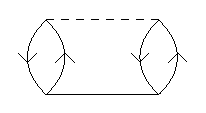
\includegraphics[scale=0.5]{graphics/ccsd_e2}}
    + \parbox{15mm}{\includegraphics[scale=0.5]{graphics/ccsd_e3}}
\end{equation*}



\end{frame}

    

\begin{frame}{Diagram rules }
    \note<6>{Filename: diagram\_rules01.tex}

    \begin{itemize}
        \item Label all lines. \pause
        \item Sum over all internal indices. \pause
        \item Extract matrix elements. 
            ($f_{\mathrm{in}}^{\mathrm{out}}$, 
            $\bra{\mathrm{lout, rout}}\ket{\mathrm{lin, rin}}$) \pause
        \item Extract cluster amplitudes with indices in the order left to right. Incoming lines are subscripts, while outgoing lines are superscripts. ($t_{\mathrm{in}}^{\mathrm{out}}$,
                        $t^{\mathrm{lout, rout}}_{\mathrm{lin, rin}}$)\pause
        \item Calculate the phase: $(-1)^{\mathrm{holelines} + \mathrm{loops}}$ \pause
        \item Multiply by a factor of $\frac{1}{2}$ for each equivalent line and each ecuivalent vertex.
    \end{itemize}

\end{frame}

    


\begin{frame}{CCSD energy equation }
    \note{Filename: ccsd\_algebraicequations02.tex}
    \begin{equation*}
    E_{CCSD} = 
    f_a^i t_i^a + \frac{1}{4} \bra{ij}\ket{ab} t_{ij}^{ab} + \frac{1}{2} \bra{ij}\ket{ab}  t_i^a  t_j^b
\end{equation*}

Note the implicit sum over repeated indices.



\end{frame}

    



\input{src/ccsd_diagramderivation02}
\begin{frame}{CCSD $\op{T}_1$ amplitude equation }
    \note{Filename: ccsd\_diagramequations02.tex}

\begin{align*}
    0 &= 
    \parbox{10mm}{\includegraphics[scale=0.4]{graphics/ccsd_hbar_04a}}
    + \parbox{18mm}{\includegraphics[scale=0.4]{graphics/ccsd_hbar_04b}}
    + \parbox{15mm}{\includegraphics[scale=0.4]{graphics/ccsd_hbar_04c}}
    + \parbox{15mm}{\includegraphics[scale=0.4]{graphics/ccsd_hbar_04d}} \\
    & \quad + \parbox{21mm}{\includegraphics[scale=0.4]{graphics/ccsd_hbar_04e}}
    + \parbox{17mm}{\includegraphics[scale=0.4]{graphics/ccsd_hbar_04f}}
    + \parbox{15mm}{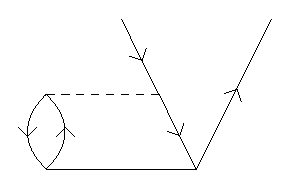
\includegraphics[scale=0.4]{graphics/ccsd_hbar_04g}}
    + \parbox{15mm}{\includegraphics[scale=0.4]{graphics/ccsd_hbar_04h}} \\
    & \quad + \parbox{17mm}{\includegraphics[scale=0.4]{graphics/ccsd_hbar_04i}}
    + \parbox{15mm}{\includegraphics[scale=0.4]{graphics/ccsd_hbar_04j}}
    + \parbox{20mm}{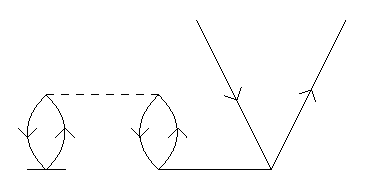
\includegraphics[scale=0.4]{graphics/ccsd_hbar_04k}}
    + \parbox{15mm}{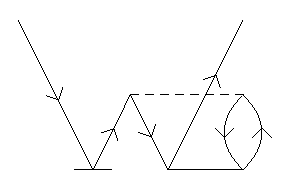
\includegraphics[scale=0.4]{graphics/ccsd_hbar_04l}} \\
    & \quad + \parbox{17mm}{\includegraphics[scale=0.4]{graphics/ccsd_hbar_04m}}
    + \parbox{15mm}{\includegraphics[scale=0.4]{graphics/ccsd_hbar_04n}}
\end{align*}

\end{frame}

    

\begin{frame}{Diagram rules }
    \note<6>{Filename: diagram\_rules01.tex}

    \begin{itemize}
        \item Label all lines. \pause
        \item Sum over all internal indices. \pause
        \item Extract matrix elements. 
            ($f_{\mathrm{in}}^{\mathrm{out}}$, 
            $\bra{\mathrm{lout, rout}}\ket{\mathrm{lin, rin}}$) \pause
        \item Extract cluster amplitudes with indices in the order left to right. Incoming lines are subscripts, while outgoing lines are superscripts. ($t_{\mathrm{in}}^{\mathrm{out}}$,
                        $t^{\mathrm{lout, rout}}_{\mathrm{lin, rin}}$)\pause
        \item Calculate the phase: $(-1)^{\mathrm{holelines} + \mathrm{loops}}$ \pause
        \item Multiply by a factor of $\frac{1}{2}$ for each equivalent line and each ecuivalent vertex.
    \end{itemize}

\end{frame}

    


\begin{frame}{CCSD $\op{T}_1$ amplitude equation }
    \note{Filename: ccsd\_algebraicequations02.tex}

\begin{align*}
    0 &= f_{i}^a + f_{e}^a t_i^e - f_{i}^mt_m^a + \bra{ma}\ket{ei} t_m^e 
        + f_{e}^m t_{im}^{ae} + \frac{1}{2} \bra{am}\ket{ef} t_{im}^{ef} \\
        &\, - \frac{1}{2} \bra{mn}\ket{ei} t_{mn}^{ea} - f_{e}^m t_i^e t_m^a
        + \bra{am}\ket{ef} t_i^e t_m^f - \bra{mn}\ket{ei} t_m^e t_n^a  \\
        & \quad + \bra{mn}\ket{ef} t_m^e t_{ni}^{fa}
        - \frac{1}{2} \bra{mn}\ket{ef} t_i^e t_{mn}^{af}
        - \frac{1}{2} \bra{mn}\ket{ef} t_n^a t_{mi}^{ef}\\
        & \quad  - \bra{mn}\ket{ef} t_i^e t_m^a t_n^f
\end{align*}


\end{frame}

    

\input{src/ccsd_diagramderivation03}
\begin{frame}{CCSD $\op{T}_2$ amplitude equation }
    \note{Filename: ccsd\_diagramequations03.tex}

\begin{align*}
    0 &= 
    \parbox{10mm}{\includegraphics[scale=0.25]{graphics/ccsd_hbar_13_01}} + 
    \parbox{10mm}{\includegraphics[scale=0.25]{graphics/ccsd_hbar_13_02}} + 
    \parbox{10mm}{\includegraphics[scale=0.25]{graphics/ccsd_hbar_13_03}} +
    \parbox{14mm}{\includegraphics[scale=0.25]{graphics/ccsd_hbar_13_04}} + 
    \parbox{14mm}{\includegraphics[scale=0.25]{graphics/ccsd_hbar_13_05}} + 
    \parbox{14mm}{\includegraphics[scale=0.25]{graphics/ccsd_hbar_13_06}} \nn
    & + \parbox{14mm}{\includegraphics[scale=0.25]{graphics/ccsd_hbar_13_07}} + 
    \parbox{14mm}{\includegraphics[scale=0.25]{graphics/ccsd_hbar_13_08}} + 
    \parbox{14mm}{\includegraphics[scale=0.25]{graphics/ccsd_hbar_13_09}} +
    \parbox{14mm}{\includegraphics[scale=0.25]{graphics/ccsd_hbar_13_10}} + 
    \parbox{14mm}{\includegraphics[scale=0.25]{graphics/ccsd_hbar_13_11}} \nn
    & + \parbox{15mm}{\includegraphics[scale=0.25]{graphics/ccsd_hbar_13_12}} +
    \parbox{19mm}{\includegraphics[scale=0.25]{graphics/ccsd_hbar_13_13}} + 
    \parbox{15mm}{\includegraphics[scale=0.25]{graphics/ccsd_hbar_13_14}} +
    \parbox{15mm}{\includegraphics[scale=0.25]{graphics/ccsd_hbar_13_15}} + 
    \parbox{15mm}{\includegraphics[scale=0.25]{graphics/ccsd_hbar_13_16}} \nn
    & + \parbox{15mm}{\includegraphics[scale=0.25]{graphics/ccsd_hbar_13_17}} +
    \parbox{17mm}{\includegraphics[scale=0.25]{graphics/ccsd_hbar_13_18}} + 
    \parbox{15mm}{\includegraphics[scale=0.25]{graphics/ccsd_hbar_13_19}} +
    \parbox{15mm}{\includegraphics[scale=0.25]{graphics/ccsd_hbar_13_20}} + 
    \parbox{15mm}{\includegraphics[scale=0.25]{graphics/ccsd_hbar_13_21}} \nn
    & + \parbox{15mm}{\includegraphics[scale=0.25]{graphics/ccsd_hbar_13_22}} + 
    \parbox{15mm}{\includegraphics[scale=0.25]{graphics/ccsd_hbar_13_23}} +
    \parbox{15mm}{\includegraphics[scale=0.25]{graphics/ccsd_hbar_13_24}} + 
    \parbox{15mm}{\includegraphics[scale=0.25]{graphics/ccsd_hbar_13_25}} +
    \parbox{15mm}{\includegraphics[scale=0.25]{graphics/ccsd_hbar_13_26}} \nn
    & + \parbox{16mm}{\includegraphics[scale=0.25]{graphics/ccsd_hbar_13_27}} +
    \parbox{17mm}{\includegraphics[scale=0.25]{graphics/ccsd_hbar_13_28}} + 
    \parbox{14mm}{\includegraphics[scale=0.25]{graphics/ccsd_hbar_13_29}} +
    \parbox{15mm}{\includegraphics[scale=0.25]{graphics/ccsd_hbar_13_30}} + 
    \parbox{15mm}{\includegraphics[scale=0.25]{graphics/ccsd_hbar_13_31}}
\end{align*}

\end{frame}

    

\begin{frame}{Diagram rules }
    \note<7>{Filename: diagram\_rules02.tex}

    \begin{itemize}
        \item Label all lines. \pause
        \item Sum over all internal indices. \pause
        \item Extract matrix elements. 
            ($f_{\mathrm{in}}^{\mathrm{out}}$, 
            $\bra{\mathrm{lout, rout}}\ket{\mathrm{lin, rin}}$) \pause
        \item Extract cluster amplitudes with indices in the order left to right. Incoming lines are subscripts, while outgoing lines are superscripts. ($t_{\mathrm{in}}^{\mathrm{out}}$,
                        $t^{\mathrm{lout, rout}}_{\mathrm{lin, rin}}$)\pause
        \item Calculate the phase: $(-1)^{\mathrm{holelines} + \mathrm{loops}}$ \pause
        \item Multiply by a factor of $\frac{1}{2}$ for each equivalent line and each ecuivalent vertex. \pause
        \item Antisymmetrize a pair of external particle/hole line that does not connect to the same operator.
    \end{itemize}

\end{frame}

    


\begin{frame}{CCSD $\op{T}_2$ amplitude equation }
    \note{Filename: ccsd\_algebraicequations03.tex}
    \scriptsize
\begin{align*}
    0 &= 
        \bra{ab} \ket{ij}
        + P(ij) \bra{ab}\ket{ej} t_i^e
        - P(ab) \bra{am} \ket{ij} t_m^b
        + P(ab) f_{e}^b t_{ij}^{ae}
        - P(ij) f_{i}^m t_{mj}^{ab} \\
        & + \, \frac{1}{2} \bra{ab}\ket{ef} t_{ij}^{ef}
        + \frac{1}{2} \bra{mn}\ket{ij} t_{mn}^{ab}
        + P(ij) P(ab) \bra{mb}\ket{ej} t_{im}^{ae} \\
        & + \, \frac{1}{2} P(ij) \bra{ab}\ket{ef} t_i^e t_j^f
        + \frac{1}{2} P(ab) \bra{mn}\ket{ij} t_m^a t_n^b
        - P(ij) P(ab) \bra{mb}\ket{ej} t_i^e t_m^a \\
        & + \, \frac{1}{4} \bra{mn}\ket{ef} t_{ij}^{ef} t_{mn}^{ab}
        + \frac{1}{2} P(ij) P(ab) \bra{mn}\ket{ef} t_{im}^{ae} t_{nj}^{fb}
        - \frac{1}{2} P(ab) \bra{mn}\ket{ef} t_{ij}^{ae} t_{mn}^{bf} \\
        & - \, \frac{1}{2} P(ij) \bra{mn}\ket{ef} t_{mi}^{ef} t_{nj}^{ab}
        - P(ij) f_{e}^m t_i^e t_{mj}^{ab}
        - P(ab) f_{e}^m t_{ij}^{ae} t_m^b \\
        & + \, P(ij) P(ab) \bra{am}\ket{ef} t_i^e t_{mj}^{fb}
        - \frac{1}{2} P(ab) \bra{am}\ket{ef} t_{ij}^{ef} t_m^b
        + P(ab) \bra{bm}\ket{ef} t_{ij}^{ae} t_m^f \\
        & - \, P(ij) P(ab) \bra{mn} \ket{ej} t_{im}^{ae} t_n^b
        + \frac{1}{2} P(ij) \bra{mn}\ket{ej} t_i^e t_{mn}^{ab}
        -P(ij) \bra{mn}\ket{ei} t_m^e t_{nj}^{ab} \\
        & - \, \frac{1}{2} P(ij) P(ab) \bra{am}\ket{ef} t_i^e t_j^f t_m^b
        + \frac{1}{2} P(ij) P(ab) \bra{mn}\ket{ej} t_i^e t_m^a t_n^b \\
        & + \, \frac{1}{4} P(ij) \bra{mn}\ket{ef} t_i^e t_{mn}^{ab} t_j^f
        - P(ij) P(ab) \bra{mn}\ket{ef} t_i^e t_m^a t_{nj}^{fb} \\
        & + \, \frac{1}{4} P(ab) \bra{mn}\ket{ef} t_m^a t_{ij}^{ef} t_n^b
        - P(ij) \bra{mn}\ket{ef} t_m^e t_i^f t_{nj}^{ab}
        - P(ab) \bra{mn}\ket{ef} t_{ij}^{ae} t_m^b t_n^f \\
        & + \, \frac{1}{4} P(ij) P(ab) \bra{mn}\ket{ef} t_i^e t_m^a t_j^f t_n^b \\
\end{align*}

\end{frame}

    

\begin{frame}{The $\barh$ expansion}
    \note{Filename: ccsd\_barh\_expansion01.tex}
        \small
        \begin{align*}
            E_{CC} &= \bra{\Psi_0}\Bigl( \hat{H}_N + \left[ \hat{H}_N, \hat{T} \right] +
                \frac{1}{2} \left[\left[ \hat{H}_N, \hat{T} \right], \hat{T}\right]
                + \frac{1}{3!} \left[ \left[\left[ \hat{H}_N, \hat{T} \right], \hat{T}\right], \hat{T} \right] \\
                & \quad + \frac{1}{4!} \left[ \left[ \left[\left[ \hat{H}_N, \hat{T} \right], \hat{T}\right], \hat{T} \right], \hat{T} \right] ++ \Bigr) \ket{\Psi_0} \\
        \end{align*}
        \begin{align*}
            0 &= \bra{\Psi_{ij\ldots}^{ab\ldots}}\Bigl( \hat{H}_N + \left[ \hat{H}_N, \hat{T} \right] +
                \frac{1}{2} \left[\left[ \hat{H}_N, \hat{T} \right], \hat{T}\right]
                + \frac{1}{3!} \left[ \left[\left[ \hat{H}_N, \hat{T} \right], \hat{T}\right], \hat{T} \right] \\
                & \quad + \frac{1}{4!} \left[ \left[ \left[\left[ \hat{H}_N, \hat{T} \right], \hat{T}\right], \hat{T} \right], \hat{T} \right] ++\Bigr) \ket{\Psi_0} \\
        \end{align*}

\end{frame}

    

\begin{frame}{The CCSD energy equation revisited}
    \note{Filename: ccsd\_barh\_expansion02.tex}
        The expanded CC energy equation involves an infinite sum over nested commutators
        \begin{align*}
            E_{CC} &= \bra{\Psi_0}\Bigl( \hat{H}_N + \left[ \hat{H}_N, \hat{T} \right] +
                \frac{1}{2} \left[\left[ \hat{H}_N, \hat{T} \right], \hat{T}\right] \\
                & \qquad + \frac{1}{3!} \left[ \left[\left[ \hat{H}_N, \hat{T} \right], \hat{T}\right], \hat{T} \right] \\
                & \qquad + \frac{1}{4!} \left[ \left[ \left[\left[ \hat{H}_N, \hat{T} \right], \hat{T}\right], \hat{T} \right], \hat{T} \right] ++ \Bigr) \ket{\Psi_0}, \\
        \end{align*}
        but fortunately we can show that it truncates naturally, depending on the Hamiltonian.
        
    \begin{block}{}
        The first term is zero by construction.
        \begin{equation*}
            \bra{\Psi_0} \op{H}_N \ket{\Psi_0} = 0
        \end{equation*}       
    \end{block}
\end{frame}

    

\begin{frame}{The CCSD energy equation revisited.}
    \note{Filename: ccsd\_barh\_expansion03.tex}
     The second term can be split up into different pieces
    \small
        \begin{align*}
        \bra{\Psi_0}\left[ \hat{H}_N, \hat{T} \right]\ket{\Psi_0} & = 
            \bra{\Psi_0} \Bigl(\left[ \hat{F}_N, \hat{T}_1 \right] + \left[ \hat{F}_N, \hat{T}_2 \right]
            + \left[ \hat{V}_N, \hat{T}_1 \right] + \left[ \hat{V}_N, \hat{T}_2 \right] \Bigr) \ket{\Psi_0}
    \end{align*}

    \begin{block}{}
    Since we need the explicit expressions for the commutators both in the next term and in the amplitude equations, we calculate them separately.
    \end{block}

\end{frame}

    

\begin{frame}{The $\barh$ expansion - $\left[ \hat{F}_N, \hat{T}_1 \right]$}
    \note{Filename: ccsd\_barh\_expansion04.tex}
    \begin{align*}
        \left[ \hat{F}_N, \hat{T}_1 \right] &= \sum_{pqia} \left(f_q^p \normord{a_p^\dagger a_q} 
            t_i^a \normord{a_a^\dagger a_i} - t_i^a \normord{a_a^\dagger a_i} f_q^p \normord{a_p^\dagger a_q} \right) \\
        &= \sum_{pqia} f_q^p t_i^a \left( \normord{a_p^\dagger a_q} \normord{a_a^\dagger a_i} -
                \normord{a_a^\dagger a_i} \normord{a_p^\dagger a_q} \right)
    \end{align*} \pause
        \begin{align*}
            \left\{a_a^\dagger a_i\right\} \left\{a_p^\dagger a_q \right\} &= \normord{a_a^\dagger a_i a_p^\dagger a_q} \pause
                = \normord{a_p^\dagger a_q a_a^\dagger a_i} \\ \pause
        \normord{a_p^\dagger a_q}\normord{a_a^\dagger a_i} &= \normord{a_p^\dagger a_q a_a^\dagger a_i}  \\ \pause
            & \quad + \normord{
               \contraction{}{a}{{}^\dagger_pa_q a^\dagger_a}{a}
                a^\dagger_p a_q a^\dagger_a a_i} +
            \normord{
                \contraction{a^\dagger_p}{a}{{}_q}{a}
                a^\dagger_p a_q a^\dagger_a a_i} \\ \pause
            & \quad + \normord{
                \contraction[1.5ex]{}{a}{{}^\dagger_pa_q a^\dagger_a}{a}
                \contraction{a^\dagger_p}{a}{{}_q}{a}
                a^\dagger_p a_q a^\dagger_a a_i} \\ \pause
            &=  \normord{a_p^\dagger a_q a_a^\dagger a_i} + \delta_{qa} \normord{a_p^\dagger a_i} + \delta_{pi} \normord{a_q a_a^\dagger}
            + \delta_{qa}\delta_{pi}
        \end{align*}
\end{frame}

    

\begin{frame}{The $\barh$ expansion - $\left[ \hat{F}_N, \hat{T}_1 \right]$}
    \note{Filename: ccsd\_barh\_expansion05.tex}

        Wicks theorem gives us
        \begin{align*}
            \left\{a_p^\dagger a_q \right\}\left\{a_a^\dagger a_i\right\} - \left\{a_a^\dagger a_i\right\} \left\{a_p^\dagger a_q \right\} &= \delta_{qa} \left\{ a_p^\dagger a_i\right\} + \delta_{pi} \left\{ a_q a_a^\dagger \right\} + \delta_{qa}\delta_{pi}.
    \end{align*}

        Inserted into the original expression, we arrive at the explicit value of the commutator
        \begin{align*}
        \left[ \hat{F}_N, \hat{T}_1 \right] &= \sum_{pai} f_a^p t_i^a \normord{a_p^\dagger a_i} + 
                \sum_{qai} f_q^i t_i^a \normord{a_q a_a^\dagger} + \sum_{ai} f_a^i t_i^a \\
            &= \left( \op{F}_N \op{T}_1 \right)_c.
        \end{align*}
    The subscript means that the product only includes terms where the operators are connected by atleast one shared index.

\end{frame}

    

\begin{frame}{The $\barh$ expansion - $\left[ \hat{F}_N, \hat{T}_2 \right]$}
    \note{Filename: ccsd\_barh\_expansion06.tex}
    \begin{align*}
        \left[ \hat{F}_N, \hat{T}_2 \right] 
        &= \left[\sum_{pq} f_q^p \normord{a^\dagger_p a_q},
            \frac{1}{4}\sum_{ijab} t_{ij}^{ab} \normord{a^\dagger_a a^\dagger_b a_j a_i} \right] \\
        &= \frac{1}{4}\sum_{\substack{pq\\ijab}}
        \left[ \normord{a^\dagger_p a_q}, \normord{a^\dagger_a a^\dagger_b a_j a_i} \right] \\
        &= \frac{1}{4}\sum_{\substack{pq\\ijab}}
            f_q^p t_{ij}^{ab}
        \left( \normord{a^\dagger_p a_q} \normord{a^\dagger_a a^\dagger_b a_j a_i}
            - \normord{a^\dagger_a a^\dagger_b a_j a_i} \normord{a^\dagger_p a_q} \right)
    \end{align*}
\end{frame}

    

\begin{frame}{The $\barh$ expansion - $\left[ \hat{F}_N, \hat{T}_2 \right]$}
    \note{Filename: ccsd\_barh\_expansion07.tex}
    \small
    \begin{align*}
        \normord{a^\dagger_a a^\dagger_b a_j a_i} \normord{a^\dagger_p a_q} &= 
            \normord{a^\dagger_a a^\dagger_b a_j a_i a^\dagger_p a_q} \\ \pause
        &= \normord{a^\dagger_p a_q a^\dagger_a a^\dagger_b a_j a_i} \pause
        \\
        \normord{a^\dagger_p a_q} \normord{a^\dagger_a a^\dagger_b a_j a_i} &= 
            \normord{a^\dagger_p a_q a^\dagger_a a^\dagger_b a_j a_i} \pause
        + \left\{ 
        \contraction{}{a}{{}^\dagger_pa_q a^\dagger_a a^\dagger_b}{a}
        a^\dagger_p a_q a^\dagger_a a^\dagger_b a_j a_i\right\}
        + \left\{ 
        \contraction{}{a}{{}^\dagger_pa_q a^\dagger_a a^\dagger_b a_j}{a}
        a^\dagger_p a_q a^\dagger_a a^\dagger_b a_j a_i\right\} \\
        & \quad 
        + \left\{ 
        \contraction{a^\dagger_p}{a}{{}_q}{a}
        a^\dagger_p a_q a^\dagger_a a^\dagger_b a_j a_i\right\}
        + \left\{ 
        \contraction{a^\dagger_p}{a}{{}_q a^\dagger_a}{a}
        a^\dagger_p a_q a^\dagger_a a^\dagger_b a_j a_i\right\} \pause
        + \left\{ 
        \contraction{a^\dagger_p}{a}{{}_q}{a}
        \contraction[1.5ex]{}{a}{{}^\dagger_pa_q a^\dagger_a a^\dagger_b}{a}
        a^\dagger_p a_q a^\dagger_a a^\dagger_b a_j a_i\right\} \\
        & \quad 
        + \left\{ 
        \contraction{a^\dagger_p}{a}{{}_q}{a}
        \contraction[1.5ex]{}{a}{{}^\dagger_pa_q a^\dagger_a a^\dagger_b a_j}{a}
        a^\dagger_p a_q a^\dagger_a a^\dagger_b a_j a_i\right\}
        + \left\{ 
        \contraction{a^\dagger_p}{a}{{}_q a^\dagger_a}{a}
        \contraction[1.5ex]{}{a}{{}^\dagger_pa_q a^\dagger_a a^\dagger_b}{a}
        a^\dagger_p a_q a^\dagger_a a^\dagger_b a_j a_i\right\}
        + \left\{ 
        \contraction{a^\dagger_p}{a}{{}_q a^\dagger_a}{a}
        \contraction[1.5ex]{}{a}{{}^\dagger_pa_q a^\dagger_a a^\dagger_b a_j}{a}
        a^\dagger_p a_q a^\dagger_a a^\dagger_b a_j a_i\right\} \\ \pause
        &= \normord{a^\dagger_p a_q a^\dagger_a a^\dagger_b a_j a_i}
        - \delta_{pj} \normord{a_q a^\dagger_a a^\dagger_b a_i}
        + \delta_{pi} \normord{a_q a^\dagger_a a^\dagger_b a_j} \\
        & \quad + \delta_{qa} \normord{a^\dagger_p a^\dagger_b a_j a_i}
        - \delta_{qb}\normord{a^\dagger_p a^\dagger_a a_j a_i} 
        - \delta_{pj} \delta_{qa} \normord{a^\dagger_b a_i} \\
        & \quad + \delta_{pi} \delta_{qa} \normord{a^\dagger_b a_j}
        + \delta_{pj} \delta_{qb} \normord{a^\dagger_a a_i}
        - \delta_{pi} \delta_{qb} \normord{a^\dagger_a a_j}
    \end{align*}

\end{frame}

    

\begin{frame}{The $\barh$ expansion - $\left[ \hat{F}_N, \hat{T}_2 \right]$}
    \note{Filename: ccsd\_barh\_expansion08.tex}
    Wicks theorem gives us
    \small
    \begin{align*}
        & \Bigl( \normord{a^\dagger_p a_q} \normord{a^\dagger_a a^\dagger_b a_j a_i}
            - \normord{a^\dagger_a a^\dagger_b a_j a_i} \normord{a^\dagger_p a_q} \Bigr) = \\
        & \qquad - \delta_{pj} \normord{a_q a^\dagger_a a^\dagger_b a_i}
        + \delta_{pi} \normord{a_q a^\dagger_a a^\dagger_b a_j}
        + \delta_{qa} \normord{a^\dagger_p a^\dagger_b a_j a_i} \\
        & \qquad - \delta_{qb}\normord{a^\dagger_p a^\dagger_a a_j a_i} 
        - \delta_{pj} \delta_{qa} \normord{a^\dagger_b a_i}
        + \delta_{pi} \delta_{qa} \normord{a^\dagger_b a_j}
        + \delta_{pj} \delta_{qb} \normord{a^\dagger_a a_i} \\
        & \qquad - \delta_{pi} \delta_{qb} \normord{a^\dagger_a a_j}
    \end{align*}
    \pause
    Inserted into the original expression, we arrive at
    \begin{align*}
        \left[ \op{F}_N, \op{T}_2 \right]
        &= \frac{1}{4} \sum_{\substack{pq\\abij}} f_q^p t_{ij}^{ab} \Bigl(
        - \delta_{pj} \normord{a_q a^\dagger_a a^\dagger_b a_i}
        + \delta_{pi} \normord{a_q a^\dagger_a a^\dagger_b a_j} \\
        & \quad + \delta_{qa} \normord{a^\dagger_p a^\dagger_b a_j a_i}
        - \delta_{qb}\normord{a^\dagger_p a^\dagger_a a_j a_i} 
        - \delta_{pj} \delta_{qa} \normord{a^\dagger_b a_i} \\
        & \quad + \delta_{pi} \delta_{qa} \normord{a^\dagger_b a_j}
        + \delta_{pj} \delta_{qb} \normord{a^\dagger_a a_i}
        - \delta_{pi} \delta_{qb} \normord{a^\dagger_a a_j} \Bigr).
    \end{align*}

\end{frame}

    

\begin{frame}{The $\barh$ expansion - $\left[ \hat{F}_N, \hat{T}_2 \right]$}
    \note{Filename: ccsd\_barh\_expansion09.tex}

    After renaming indices and changing the order of operators, we arrive at the explicit expression
    \begin{align*}
        \left[ \op{F}_N, \op{T}_2 \right]
        &= \frac{1}{2} \sum_{qijab} f_q^i t_{ij}^{ab} \normord{a_q a^\dagger_a a^\dagger_b a_j}
        + \frac{1}{2} \sum_{pijab} f_a^p t_{ij}^{ab} \normord{a^\dagger_p a^\dagger_b a_j a_i} \\
        & \quad + \sum_{ijab} f_a^i t_{ij}^{ab} \normord{a^\dagger_b a_j} \\
    &= \left( \op{F}_N \op{T}_2\right)_c.
    \end{align*}
    The subscript implies that only the connected terms from the product contribute.

\end{frame}

    

\begin{frame}{The $\barh$ expansion - $\frac{1}{2}\left[ \left[ \op{F}_N, \op{T}_1 \right], \op{T}_1 \right]$}
    \note{Filename: ccsd\_barh\_expansion10.tex}
    \small
        \begin{align*}
        \left[ \hat{F}_N, \hat{T}_1 \right] &= \sum_{pai} f_a^p t_i^a \normord{a_p^\dagger a_i} + 
                \sum_{qai} f_q^i t_i^a \normord{a_q a_a^\dagger} + \sum_{ai} f_a^i t_i^a
        \end{align*}

        \pause
    \begin{align*}
        \left[ \left[ \op{F}_N, \op{T}_1 \right], \op{T}_1\right] 
        &= \Bigl[ \sum_{pai} f_a^p t_i^a \normord{a_p^\dagger a_i} +
            \sum_{qai} f_q^i t_i^a \normord{a_q a_a^\dagger} + \sum_{ai} f_a^i t_i^a, \sum_{jb} t_j^b \normord{a_b^\dagger a_j} \\
        &= \Bigl[ \sum_{pai} f_a^p t_i^a \normord{a_p^\dagger a_i} +
            \sum_{qai} f_q^i t_i^a \normord{a_q a_a^\dagger}, \sum_{jb} t_j^b \normord{a_b^\dagger a_j} \\
        &= \sum_{pabij} f_a^p t_i^a t_j^b \left[ \normord{a_p^\dagger a_i}, \normord{a_b^\dagger a_j} \right] +
            \sum_{qabij} f_q^i t_i^a t_j^b \left[ \normord{a_q a_a^\dagger}, \normord{a_b^\dagger a_j} \right]
    \end{align*}
        \pause
    \begin{align*}
        \normord{a_b^\dagger a_j} \normord{a_p^\dagger a_i} &= \normord{a_b^\dagger a_j a_p^\dagger a_i} 
            = \normord{ a_p^\dagger a_i a_b^\dagger a_j} \\
        \pause
        \normord{a_b^\dagger a_j} \normord{a_q a_a^\dagger} &= \normord{ a_b^\dagger a_j a_q a_a^\dagger} 
            =  \normord{ a_q a_a^\dagger a_b^\dagger a_j}
    \end{align*}
\end{frame}

    

\begin{frame}{The $\barh$ expansion - $\left[ \left[ \op{F}_N, \op{T}_1 \right], \op{T}_1 \right]$}
    \note{Filename: ccsd\_barh\_expansion11.tex}

    \small
    \begin{align*}
        \frac{1}{2} \left[ \left[ \op{F}_N, \op{T}_1 \right], \op{T}_1\right] 
        &= \frac{1}{2} \left(\sum_{pabij} f_a^p t_i^a t_j^b \delta_{pj} \normord{a_i a_b^\dagger}
            - \sum_{qabij} f_q^i t_i^a t_j^b \delta_{qb} \normord{a_a^\dagger a_j}\right) \\
        &= -\frac{1}{2} 2 \sum_{abij} f_b^j t_j^a t_i^b \normord{a_a^\dagger a_i} \\
        &= -\sum_{abij} f_b^j t_j^a t_i^b \normord{a_a^\dagger a_i} \\
        &= \frac{1}{2} \left(  \op{F}_N \op{T}_1^2 \right)_c
    \end{align*}

\end{frame}

    

\begin{frame}{The CCSD energy equation revisited }
    \note{Filename: ccsd\_barh\_expansion12.tex}

    \small
    \begin{align*}
        \bra{\Phi_0} \left[ \hat{V}_N, \hat{T}_1 \right] \ket{\Phi_0} &= 
            \bra{\Phi_0}
                \left[ \frac{1}{4} \sum_{pqrs} \bra{pq}\ket{rs} \normord{a^\dagger_p a^\dagger_q a_s  a_r},
                    \sum_{ia} t_i^a \normord{a^\dagger_a a_i} \right] \ket{\Phi_0} \\ \pause
            &= \frac{1}{4}\sum_{\substack{
                pqr \\
                sia}} \bra{pq}\ket{rs} t_i^a \bra{\Phi_0} 
                \left[ \normord{a^\dagger_p a^\dagger_q a_s  a_r}, \normord{a^\dagger_a a_i} \right]
                \ket{\Phi_0} \\ \pause
        &= 0
    \end{align*}



\end{frame}

    

\begin{frame}{The CCSD energy equation revisited }
    \note{Filename: ccsd\_barh\_expansion13.tex}

    \small
    \begin{align*}
        & \bra{\Phi_0} \left[ \hat{V}_N, \hat{T}_2 \right] \ket{\Phi_0}= \\
            & \quad \bra{\Phi_0}
                \left[ \frac{1}{4} \sum_{pqrs} \bra{pq}\ket{rs} \normord{a^\dagger_p a^\dagger_q a_s  a_r},
                    \frac{1}{4}\sum_{ijab} t_{ij}^{ab} \normord{a^\dagger_a a^\dagger_b a_j a_i} \right] \ket{\Phi_0} \\ \pause
            &= \frac{1}{16}\sum_{\substack{
                    pqr \\
                    sijab}} \bra{pq}\ket{rs}t_{ij}^{ab} \bra{\Phi_0} 
                \left[ \normord{a^\dagger_p a^\dagger_q a_s  a_r}, \normord{a^\dagger_a a^\dagger_b a_j a_i} \right]
                \ket{\Phi_0} \\ \pause
            &= \frac{1}{16}\sum_{\substack{
                    pqr \\
                    sijab}} \bra{pq}\ket{rs}t_{ij}^{ab} \bra{\Phi_0}
            \Bigl(
            \left\{
            \contraction{a^\dagger_p a^\dagger_q a_s}{a}{{}_r}{a}
            \contraction[1.25ex]{a^\dagger_p a^\dagger_q}{a}{{}_s a_r a^\dagger_a}{a}
            \contraction[1.50ex]{a^\dagger_p}{a}{{}^\dagger_q a_s a_r a^\dagger_a a^\dagger_b}{a}
            \contraction[1.75ex]{}{a}{{}^\dagger_p a^\dagger_q a_s a_r a^\dagger_a a^\dagger_b a_j}{a}
            a^\dagger_p a^\dagger_q a_s  a_r a^\dagger_a a^\dagger_b a_j a_i \right\}
            + \left\{
            \contraction{a^\dagger_p a^\dagger_q}{a}{{}_s a_r}{a}
            \contraction[1.25ex]{a^\dagger_p a^\dagger_q a_s}{a}{{}_r a^\dagger_p}{a}
            \contraction[1.50ex]{a^\dagger_p}{a}{{}^\dagger_q a_s a_r a^\dagger_a a^\dagger_b}{a}
            \contraction[1.75ex]{}{a}{{}^\dagger_p a^\dagger_q a_s a_r a^\dagger_a a^\dagger_b a_j}{a}
            a^\dagger_p a^\dagger_q a_s  a_r a^\dagger_a a^\dagger_b a_j a_i \right\} \\
            & \quad \left\{
            \contraction{a^\dagger_p a^\dagger_q a_s}{a}{{}_r}{a}
            \contraction[1.25ex]{a^\dagger_p a^\dagger_q}{a}{{}_s a_r a^\dagger_a}{a}
            \contraction[1.5ex]{}{a}{{}^\dagger_p a^\dagger_q a_s a_r a^\dagger_a a^\dagger_b}{a}
            \contraction[1.75ex]{a^\dagger_p}{a}{{}^\dagger_q a_s a_r a^\dagger_a a^\dagger_b a_j}{a}
            a^\dagger_p a^\dagger_q a_s  a_r a^\dagger_a a^\dagger_b a_j a_i \right\}
            + \left\{
            \contraction{a^\dagger_p a^\dagger_q}{a}{{}_s a_r}{a}
            \contraction[1.25ex]{a^\dagger_p a^\dagger_q a_s}{a}{{}_r a^\dagger_p}{a}
            \contraction[1.5ex]{}{a}{{}^\dagger_p a^\dagger_q a_s a_r a^\dagger_a a^\dagger_b}{a}
            \contraction[1.75ex]{a^\dagger_p}{a}{{}^\dagger_q a_s a_r a^\dagger_a a^\dagger_b a_j}{a}
            a^\dagger_p a^\dagger_q a_s  a_r a^\dagger_a a^\dagger_b a_j a_i \right\}
            \Bigr) \ket{\Phi_0} \\ \pause
            &= \frac{1}{4} \sum_{ijab} \bra{ij}\ket{ab} t_{ij}^{ab}
    \end{align*}


\end{frame}

    

\begin{frame}{The CCSD energy equation revisited }
    \note{Filename: ccsd\_barh\_expansion14.tex}

    The CCSD energy get two contributions from $\left(\op{H}_N \op{T}\right)_c$
    \begin{align*}
        E_{CC} & \Leftarrow \bra{\Phi_0} \left[ \hat{H}_N, \hat{T} \right] \ket{\Phi_0} \\
            &= \sum_{ia} f_a^i t_i^a + \frac{1}{4} \sum_{ijab} \bra{ij}\ket{ab} t_{ij}^{ab}
    \end{align*}



\end{frame}

    

\begin{frame}{The CCSD energy equation revisited }
    \note{Filename: ccsd\_barh\_expansion15.tex}

    \begin{align*}
        E_{CC} & \Leftarrow \bra{\Phi_0} \frac{1}{2} \left( \op{H}_N \op{T}^2 \right)_c \ket{\Phi_0}
     \end{align*}
    \pause
    \small
    \begin{align*}
        & \bra{\Phi_0} \frac{1}{2} \left( \op{V}_N \op{T}_1^2 \right)_c \ket{\Phi_0} = \\
            & \quad \frac{1}{8} \sum_{pqrs} \sum_{ijab} \bra{pq}\ket{rs} t_i^a t_j^b 
            \bra{\Phi_0} \left(\normord{a^\dagger_p a^\dagger_q a_s  a_r} 
            \normord{a^\dagger_a a_i} \normord{a^\dagger_b a_j} \right)_c\ket{\Phi_0} \\ \pause
        &= \frac{1}{8} \sum_{pqrs} \sum_{ijab} \bra{pq}\ket{rs} t_i^a t_j^b \bra{\Phi_0} \\
        & \quad \Bigl( 
        \left\{
        \contraction{a^\dagger_p a^\dagger_q a_s}{a}{{}_r}{a}
        \contraction[1.25ex]{a^\dagger_p}{a}{{}^\dagger_q a_s a_r a^\dagger_a}{a}
        \contraction[1.5ex]{a^\dagger_p a^\dagger_q }{a}{{}_s a_r a^\dagger_a a_i}{a}
        \contraction[1.75ex]{}{a}{{}^\dagger_p a^\dagger_q a_s a_r a^\dagger_a a_i a^\dagger_b}{a}
        a^\dagger_p a^\dagger_q a_s  a_r a^\dagger_a a_i a^\dagger_b a_j \right\}
        +\left\{
        \contraction{a^\dagger_p a^\dagger_q}{a}{{}_s a_r}{a}
        \contraction[1.25ex]{a^\dagger_p}{a}{{}^\dagger_q a_s a_r a^\dagger_a}{a}
        \contraction[1.5ex]{a^\dagger_p a^\dagger_q a_s}{a}{{}_r a^\dagger_a a_i}{a}
        \contraction[1.75ex]{}{a}{{}^\dagger_p a^\dagger_q a_s a_r a^\dagger_a a_i a^\dagger_b}{a}
        a^\dagger_p a^\dagger_q a_s  a_r a^\dagger_a a_i a^\dagger_b a_j \right\}
        + \left\{
        \contraction{a^\dagger_p a^\dagger_q a_s}{a}{{}_r}{a}
        \contraction[1.25ex]{}{a}{{}^\dagger_p q^\dagger_q a_s a_r a^\dagger_a}{a}
        \contraction[1.5ex]{a^\dagger_p a^\dagger_q }{a}{{}_s a_r a^\dagger_a a_i}{a}
        \contraction[1.75ex]{a^\dagger_p}{a}{{}^\dagger_q a_s a_r a^\dagger_a a_i a^\dagger_b}{a}
        a^\dagger_p a^\dagger_q a_s  a_r a^\dagger_a a_i a^\dagger_b a_j \right\} \\
        & \quad +\left\{
        \contraction{a^\dagger_p a^\dagger_q}{a}{{}_s a_r}{a}
        \contraction[1.25ex]{}{a}{{}^\dagger_p q^\dagger_q a_s a_r a^\dagger_a}{a}
        \contraction[1.5ex]{a^\dagger_p a^\dagger_q a_s}{a}{{}_r a^\dagger_a a_i}{a}
        \contraction[1.75ex]{a^\dagger_p}{a}{{}^\dagger_q a_s a_r a^\dagger_a a_i a^\dagger_b}{a}
        a^\dagger_p a^\dagger_q a_s  a_r a^\dagger_a a_i a^\dagger_b a_j \right\}
        \Bigr) \ket{\Phi_0} \\ \pause
        &= \frac{1}{2} \sum_{ijab} \bra{ij}\ket{ab} t_i^a t_j^b
    \end{align*}



\end{frame}

    

\begin{frame}{The CCSD energy equation revisited }
    \note{Filename: ccsd\_barh\_expansion16.tex}

    \begin{itemize}
        \item No contractions possible between cluster operators. \pause
        \item Cluster operators need to contract with free indices to the left. \pause
        \item Disconnected parts automatically cancel in the commutator. \pause
        \item Onebody operators can connect to maximum two cluster operators. \pause
        \item Twobody operators can connect to maximum four cluster operators. \pause
        \item Different terms in the $\barh$ expansion contributes to different equations.
    \end{itemize}


\end{frame}

    


\begin{frame}
    \frametitle{Factoring, motivation}
\note{Filename: ccsd\_factoring01.tex}

\small
\begin{block}{Diagram (2.12)}
    \begin{equation*}
        \parbox{40mm}{\includegraphics[scale=0.5]{graphics/ccsd_hbar_13_12}}
        = \frac{1}{4}  \bra{mn}\ket{ef} t_{ij}^{ef} t_{mn}^{ab}
    \end{equation*}
\end{block}
\begin{block}{Diagram (2.26)}
    \begin{equation*}
        \parbox{40mm}{\includegraphics[scale=0.5]{graphics/ccsd_hbar_13_26}}
        = \frac{1}{4} P(ij) \bra{mn}\ket{ef} t_i^e t_{mn}^{ab} t_j^f
    \end{equation*}
\end{block}
\begin{block}{Diagram (2.31)}
    \begin{equation*}
        \parbox{40mm}{\includegraphics[scale=0.5]{graphics/ccsd_hbar_13_31}}
        = \frac{1}{4} P(ij) P(ab) \bra{mn}\ket{ef} t_i^e t_m^a t_j^f t_n^b
    \end{equation*}
\end{block}
\end{frame}


\begin{frame}
    \frametitle{Factoring, motivation}
\note{Filename: ccsd\_factoring02.tex}

\scriptsize
\begin{block}{Diagram (2.12)}
    \begin{equation*}
        \parbox{40mm}{\includegraphics[scale=0.5]{graphics/ccsd_hbar_13_12}}
        = \frac{1}{4}  \bra{mn}\ket{ef} t_{ij}^{ef} t_{mn}^{ab}
    \end{equation*}
\end{block}
Diagram cost: $n_p^4 n_h^4$
\begin{block}{Diagram (2.13) - Factored}
\small
    \begin{align*}
        \parbox{40mm}{\includegraphics[scale=0.5]{graphics/ccsd_hbar_13_12}}
        &= \frac{1}{4}  \bra{mn}\ket{ef} t_{ij}^{ef} t_{mn}^{ab} \nn
        &= \frac{1}{4}  \left(\bra{mn}\ket{ef} t_{ij}^{ef}\right)  t_{mn}^{ab} \nn
        &= \frac{1}{4} X_{ij}^{mn} t_{mn}^{ab}
    \end{align*}
\end{block}
\end{frame}


\begin{frame}
    \frametitle{Factoring, motivation}
\note{Filename: ccsd\_factoring03.tex}

\small
\begin{block}{Diagram (2.26)}
    \begin{align*}
        \parbox{40mm}{\includegraphics[scale=0.5]{graphics/ccsd_hbar_13_26}}
        &= \frac{1}{4} P(ij) \bra{mn}\ket{ef} t_i^e t_{mn}^{ab} t_j^f
    \end{align*}
\end{block}
Diagram cost: $n_p^4 n_h^4$
\begin{block}{Diagram (2.26) - Factored}
    \begin{align*}
        \parbox{40mm}{\includegraphics[scale=0.5]{graphics/ccsd_hbar_13_26}}
        &= \frac{1}{4} P(ij) \bra{mn}\ket{ef} t_i^e t_{mn}^{ab} t_j^f \nn
        &= \frac{1}{4} P(ij) t_{mn}^{ab} t_i^e X_{ej}^{mn} \nn
        &= \frac{1}{4} P(ij) t_{mn}^{ab} Y^{mn}_{ij}
    \end{align*}
\end{block}
\end{frame}



\begin{frame}
    \frametitle{Factoring, motivation}
\note{Filename: ccsd\_factoring04.tex}

\scriptsize
\begin{block}{Diagram (2.31)}
    \begin{align*}
        \parbox{40mm}{\includegraphics[scale=0.5]{graphics/ccsd_hbar_13_31}}
        &= \frac{1}{4} P(ij) P(ab) \bra{mn}\ket{ef} t_i^e t_m^a t_j^f t_n^b
    \end{align*}
\end{block}
Diagram cost: $n_p^4 n_h^4$
\begin{block}{Diagram (2.31) - Factored}
    \begin{align*}
        \parbox{40mm}{\includegraphics[scale=0.4]{graphics/ccsd_hbar_13_31}}
        &= \frac{1}{4} P(ij) P(ab) \bra{mn}\ket{ef} t_i^e t_m^a t_j^f t_n^b \nn
        &= \frac{1}{4} P(ij) P(ab) t_m^a t_n^b t_i^e X_{ej}^{mn} \nn
        &= \frac{1}{4} P(ij) P(ab) t_m^a t_n^b Y_{ij}^{mn} \nn
        &= \frac{1}{4} P(ij) P(ab) t_m^a Z_{ij}^{mb}
    \end{align*}
\end{block}
\end{frame}

\begin{frame}
    \frametitle{Factoring, Classification}
\note{Filename: ccsd\_factoring05.tex}

A diagram is classified by how many hole and particle lines between a $\hat{T}_i$ operator and the interaction ($T_i(p^{np} h^{nh})$).
\begin{block}{Diagram (2.12) Classification}
    \begin{equation*}
        \parbox{40mm}{\includegraphics[scale=0.5]{graphics/ccsd_hbar_13_12}}
        = \frac{1}{4}  \bra{mn}\ket{ef} t_{ij}^{ef} t_{mn}^{ab}
    \end{equation*}
\end{block}
This diagram is classified as $T_2(p^2) \times T_2(h^2)$
\end{frame}



\begin{frame}
    \frametitle{Factoring, Classification}
\note{Filename: ccsd\_factoring06.tex}

\begin{block}{Diagram (2.26)} 
    \begin{equation*}
        \parbox{40mm}{\includegraphics[scale=0.5]{graphics/ccsd_hbar_13_26}}
        = \frac{1}{4} P(ij) \bra{mn}\ket{ef} t_i^e t_{mn}^{ab} t_j^f
    \end{equation*}
\end{block}
This diagram is classified as $T_2(h^2) \times T_1(p) \times T_1(p)$
\begin{block}{Diagram (2.31)} 
    \begin{equation*}
        \parbox{40mm}{\includegraphics[scale=0.5]{graphics/ccsd_hbar_13_31}}
        = \frac{1}{4} P(ij) P(ab) \bra{mn}\ket{ef} t_i^e t_m^a t_j^f t_n^b
    \end{equation*}
\end{block}
This diagram is classified as $T_1(p) \times T_1(p) \times T_1(h) \times T_1(h)$
\end{frame}


\begin{frame}
    \frametitle{Factoring, Classification}
\note{Filename: ccsd\_factoring07.tex}

\begin{block}{\centering Cost of making intermediates}
\begin{center}
\begin{tabular}{|l||c|c|}
    \hline
    Object & CPU cost & Memory cost \\
    \hline
    $T_2(h)$ & $n_p^2 n_h$ & $ n_p^2$ \\
    \hline
    $T_2(h^2)$ & $n_p^2$ & $ n_h^{-2} n_p^2$ \\
    \hline
    $T_2(p)$ & $n_p n_h^2$ & $ n_h^2$ \\
    \hline
    $T_2(ph)$ & $n_p n_h$ & $1$ \\
    \hline
    $T_1(h)$ & $n_p$ & $ n_h^{-1} n_p$ \\
    \hline
    $T_2(ph^2)$ & $n_p$ & $ n_h^{-2}$ \\
    \hline
    $T_2(p^2)$ & $ n_h^2$ & $ n_p^{-2} n_h^2$ \\
    \hline
    $T_1(p)$ & $n_h$ & $ n_p^{-1} n_h$ \\
    \hline
    $T_2(p^2h)$ & $n_h$ & $ n_p^{-2}$ \\
    \hline
    $T_1(ph)$ & $1$ & $ n_p^{-1} n_h^{-1}$ \\
    \hline
\end{tabular}
\end{center}

\end{block}
\end{frame}


\begin{frame}
    \frametitle{Factoring, Classification}
\note{Filename: ccsd\_factoring11.tex}

\begin{block}{Classification of $\hat{T}_1$ diagrams}
\begin{tabular}{|l||l|}
    \hline
    Object & Expression id \\
    \hline
    $T_2(ph)$ & 5, 11\\
    \hline
    $T_1(h)$ & 3, 8, 10, 13, 14\\
    \hline
    $T_2(ph^2)$ & 7, 12\\
    \hline
    $T_1(p)$ & 2, 8, 9, 12, 14 \\
    \hline
    $T_2(p^2h)$ & 6, 13\\
    \hline
    $T_1(ph)$ & 4, 9, 10, 11, 14\\
    \hline
\end{tabular}

\end{block}
\end{frame}



\begin{frame}
    \frametitle{Factoring, Classification}
\note{Filename: ccsd\_factoring08.tex}

\begin{block}{Classification of $\hat{T}_2$ diagrams}
\small
\begin{tabular}{|l||l|}
    \hline
    Object & Expression id \\
    \hline
    $T_2(h)$ & 5, 15, 16, 23, 29 \\
    \hline
    $T_2(h^2)$ & 7, 12, 22, 26 \\
    \hline
    $T_2(p)$ & 4, 14, 17, 20, 30 \\
    \hline
    $T_2(ph)$ & 8, 13, 13, 18, 21, 27 \\
    \hline
    $T_1(h)$ & 3, 10, 10, 11, 17, 19, 21, 24, 25, 25, 27, 28, 28, 30, 31, 31 \\
    \hline
    $T_2(ph^2)$ & 14 \\
    \hline
    $T_2(p^2)$ & 6, 12, 19, 28 \\
    \hline
    $T_1(p)$ & 2, 9, 9, 11, 16, 18, 22, 24, 24, 25, 26, 26, 27, 29, 31, 31 \\
    \hline
    $T_2(p^2h)$ & 15 \\
    \hline
    $T_1(ph)$ & 20, 23, 29, 30 \\
    \hline
\end{tabular}

\end{block}
\end{frame}



\begin{frame}
    \frametitle{Factoring, $T_2(h)$}
\note{Filename: ccsd\_factoring09.tex}

\begin{block}{Contribution to the $\hat{T}_2$ amplitude equation from $T_2(h)$}
\begin{align*}
    T_2(h) & \Leftarrow 
        - P(ij) f_{i}^m t_{mj}^{ab}
        - \frac{1}{2} P(ij) \bra{mn}\ket{ef} t_{mi}^{ef} t_{nj}^{ab}
        - P(ij) f_{e}^m t_i^e t_{mj}^{ab} \nn
        & \quad - P(ij) \bra{mn}\ket{ei} t_m^e t_{nj}^{ab}
        - P(ij) \bra{mn}\ket{ef} t_m^e t_i^f t_{nj}^{ab} \nn
    & = - P(ij) t_{im}^{ab} \Bigl[ 
        f_j^m 
        + \bra{mn}\ket{je} t_n^e
        + \frac{1}{2} \bra{mn}\ket{ef}  t_{jn}^{ef} \nn
        & \quad + t_j^e \Bigl(
            f_e^m 
            + \bra{mn}\ket{ef} t_n^f
        \Bigr)
    \Bigr] \nn
    & = - P(ij) t_{im}^{ab} (\mathrm{\bar{H}3})_j^m
\end{align*}

\end{block}
\end{frame}


\begin{frame}
    \frametitle{Factoring, $T_2(h^2)$}
\note{Filename: ccsd\_factoring10.tex}

\begin{block}{Contribution to the $\hat{T}_2$ amplitude equation from $T_2(h^2)$}
\begin{align*}
    T_2(h^2) & \Leftarrow
        \frac{1}{2} \bra{mn}\ket{ij} t_{mn}^{ab}
        + \frac{1}{4} \bra{mn}\ket{ef} t_{ij}^{ef} t_{mn}^{ab}
        + \frac{1}{2} P(ij) \bra{mn}\ket{ej} t_i^e t_{mn}^{ab} \nn
        & \quad + \frac{1}{4} P(ij) \bra{mn}\ket{ef} t_i^e t_{mn}^{ab} t_j^f \nn
    &= \frac{1}{2} t_{mn}^{ab} \Bigl[
        \bra{mn}\ket{ij}
        + \frac{1}{2} \bra{mn}\ket{ef} t_{ij}^{ef} \nn
        & \quad + P(ij) t_j^e \Bigl(
            \bra{mn}\ket{ie} + \frac{1}{2} \bra{mn}\ket{fe} t_i^f
        \Bigr)
    \Bigr] \nn
    &= \frac{1}{2} t_{mn}^{ab} (\mathrm{\bar{H}9})_{ij}^{mn}
\end{align*}

\end{block}
\end{frame}


\begin{frame}
    \frametitle{Factored $T_1$ amplitude equations}
\note{Filename: ccsd\_factoring12.tex}

\begin{align*}
    0 &= f_{i}^a + \bra{ma}\ket{ei} t_m^e + \frac{1}{2} \bra{am}\ket{ef} t_{im}^{ef}
        + t_i^e (\mathrm{I2a})_e^a - t_m^a (\mathrm{\bar{H}3})_i^m \nn
    & \quad + \frac{1}{2} t_{mn}^{ea} (\mathrm{\bar{H}7})_{ie}^{mn} + t_{im}^{ae} 
        (\mathrm{\bar{H}1})_e^m \nn
\end{align*}

Can be solved by
\begin{enumerate}
\item Matrix inversion for each iteration ($n_p^3 n_h^3$)
\item Extracting diagonal elements ($n_p^3 n_h^2$)
\end{enumerate}
\end{frame}


\begin{frame}
    \frametitle{Factored $T_1$ amplitude equations}
\note{Filename: ccsd\_factoring13.tex}

\begin{align*}
    0 &= f_{i}^a + \bra{ma}\ket{ei} t_m^e + \frac{1}{2} \bra{am}\ket{ef} t_{im}^{ef}
        + t_i^e (\mathrm{I2a})_e^a - t_m^a (\mathrm{\bar{H}3})_i^m \nn
    & \quad + \frac{1}{2} t_{mn}^{ea} (\mathrm{\bar{H}7})_{ie}^{mn} + t_{im}^{ae} 
        (\mathrm{\bar{H}1})_e^m \nn \pause
    &= f_{i}^a + \bra{ma}\ket{ei} t_m^e
        + t_i^a (\mathrm{I2a})_a^a + (1 - \delta_{ea}) t_i^e (\mathrm{I2a})_e^a \nn
    & \quad - t_i^a (\mathrm{\bar{H}3})_i^i - (1 - \delta_{mi}) t_m^a (\mathrm{\bar{H}3})_i^m 
        + \frac{1}{2} \bra{am}\ket{ef} t_{im}^{ef} + \frac{1}{2} t_{mn}^{ea} (\mathrm{\bar{H}7})_{ie}^{mn} \nn
    & \quad + t_{im}^{ae} (\mathrm{\bar{H}1})_e^m \nn \pause
    &= f_{i}^a + t_i^a \Bigl( (\mathrm{I2a})_a^a - (\mathrm{\bar{H}3})_i^i \Bigr)
        + \bra{ma}\ket{ei} t_m^e \nn
    & \quad + (1 - \delta_{ea}) t_i^e (\mathrm{I2a})_e^a - (1 - \delta_{mi}) t_m^a (\mathrm{\bar{H}3})_i^m
        + \frac{1}{2} \bra{am}\ket{ef} t_{im}^{ef} \nn
    & \quad + \frac{1}{2} t_{mn}^{ea} (\mathrm{\bar{H}7})_{ie}^{mn} + t_{im}^{ae} (\mathrm{\bar{H}1})_e^m \nn
\end{align*}
\end{frame}




\begin{frame}
    \frametitle{Factored $T_1$ amplitude equations}
\note{Filename: ccsd\_factoring14.tex}

    Define
\begin{equation*}
    D_i^a = (\mathrm{\bar{H}3})_i^i - (\mathrm{I2a})_a^a,
\end{equation*}
and we get the $T_1$ amplitude equations
\begin{align*}
    D_i^a t_i^a &= 
        f_{i}^a + \bra{ma}\ket{ei} t_m^e+ (1 - \delta_{ea}) t_i^e (\mathrm{I2a})_e^a & \\
    & \quad - (1 - \delta_{mi}) t_m^a (\mathrm{\bar{H}3})_i^m
        + \frac{1}{2} \bra{am}\ket{ef} t_{im}^{ef} \nn
    & \quad + \frac{1}{2} t_{mn}^{ea} (\mathrm{\bar{H}7})_{ie}^{mn} + t_{im}^{ae} (\mathrm{\bar{H}1})_e^m.
\end{align*}
\end{frame}




\begin{frame}
    \frametitle{Factored $T_2$ amplitude equations}
\note{Filename: ccsd\_factoring15.tex}

\begin{align*}
    0 &= \bra{ab} \ket{ij}
        + \frac{1}{2} \bra{ab}\ket{ef} t_{ij}^{ef}
        - P(ij) t_{im}^{ab} (\mathrm{\bar{H}3})_j^m
        + \frac{1}{2} t_{mn}^{ab} (\mathrm{\bar{H}9})_{ij}^{mn} \\
        & \quad + P(ab) t_{ij}^{ae} (\mathrm{\bar{H}2})_e^b
        + P(ij) P(ab) t_{im}^{ae} (\mathrm{I10c})_{ej}^{mb}
        - P(ab) t_m^a (\mathrm{I12a})_{ij}^{mb} \\
        & \quad + P(ij)t_i^e (\mathrm{I}11a)_{ej}^{ab} 
\end{align*}

Can be solved by
\begin{enumerate}
\item Matrix inversion for each iteration ($n_p^6 n_h^6$)
\item Extracting diagonal elements ($n_p^4 n_h^2$)
\end{enumerate}
\end{frame}


\begin{frame}
    \frametitle{Factored $T_2$ amplitude equations}
\note{Filename: ccsd\_factoring16.tex}

Similarily we define
\begin{equation*}
    D_{ij}^{ab} = (\mathrm{\bar{H}3})_i^i + (\mathrm{\bar{H}3})_j^j
        - (\mathrm{\bar{H}2})_a^a - (\mathrm{\bar{H}2})_b^b 
\end{equation*}
and get the $T_2$ amplitude equations
\begin{equation*}
\begin{split}
    D_{ij}^{ab} t_{ij}^{ab} &= 
        \bra{ab} \ket{ij} 
        + \frac{1}{2} \bra{ab}\ket{ef} t_{ij}^{ef}
        - P(ij)(1-\delta_{jm}) t_{im}^{ab} (\mathrm{\bar{H}3})_j^m \\
        & \quad + \frac{1}{2} t_{mn}^{ab} (\mathrm{\bar{H}9})_{ij}^{mn}
        + P(ab) (1-\delta_{be}) t_{ij}^{ae} (\mathrm{\bar{H}2})_e^b \\
        & \quad + P(ij) P(ab) t_{im}^{ae} (\mathrm{I10c})_{ej}^{mb}
        - P(ab) t_m^a (\mathrm{I12a})_{ij}^{mb} \\
        & \quad + P(ij)t_i^e (\mathrm{I}11a)_{ej}^{ab}
\end{split}
\end{equation*}

\end{frame}



\begin{frame}
\frametitle{Coupled Cluster algorithm}
\note{Filename: ccsd\_algorithm01.tex}
\begin{center}
\begin{fmpage}{7.7cm}
\hspace*{0.4cm} Setup modelspace \\ 
\hspace*{0.4cm} Calculate f and v amplitudes \\
\hspace*{0.4cm} $t_i^a \gets 0$; $t_{ij}^{ab} \gets 0$ \\
\hspace*{0.4cm} $E \gets 1$; $E_{old} \gets 0$ \\ \pause
\hspace*{0.4cm} $E_{ref} \gets \sum_{i} \bra{i} \op{t} \ket{i} +
    \frac{1}{2} \sum_{ij} \bra{ij} \op{v} \ket{ij}$ \\ \pause
\hspace*{0.4cm} while not converged $(E - E_{old} > \epsilon)$ \\ \pause
\hspace*{0.8cm} Calculate intermediates \\ \pause
\hspace*{0.8cm} $t_i^a \gets $ calculated value \\
\hspace*{0.8cm} $t_{ij}^{ab} \gets $ calculated value \\ \pause
\hspace*{0.8cm} $E_{old} \gets E$ \\
\hspace*{0.8cm} $E \gets f_a^i t_i^a + \frac{1}{4} \bra{ij}\ket{ab} t_{ij}^{ab} + \frac{1}{2} \bra{ij}\ket{ab}  t_i^a  t_j^b$ \\ \pause
\hspace*{0.4cm} end while \\
\hspace*{0.4cm} $E_{GS} \gets E_{ref} + E$
\end{fmpage}
\end{center}
\end{frame}

%\begin{frame}
\frametitle{Coupled Cluster algorithm}
\note{Filename: ccsd\_algorithm02.tex}

Typical convergence of the $T_2$ amplitudes
\begin{center}
    \includegraphics[scale=0.3]{../graphics/He4-convergence-N2}
\end{center}
\end{frame}






\end{document}



\frame
{
\frametitle{Schr\"odinger picture}
\begin{small}
{\scriptsize
The time-dependent Schr\"odinger equation (or equation of motion) reads
\[
\imath \hbar\frac{\partial }{\partial t}|\Psi_S(t)\rangle = \hat{H}\Psi_S(t)\rangle,
\]
where the subscript $S$ stands for Schr\"odinger here.
A formal solution is given by 
\[
|\Psi_S(t)\rangle = \exp{(-\imath\hat{H}(t-t_0)/\hbar)}|\Psi_S(t_0)\rangle.
\]
The Hamiltonian $\hat{H}$ is hermitian and the exponent represents a unitary 
operator with an operation carried ut on the wave function at a time $t_0$.
}
\end{small}
}

\frame
{
\frametitle{Interaction picture}
\begin{small}
{\scriptsize
Our Hamiltonian is normally written out as the sum of an unperturbed part $\hat{H}_0$ and an interaction part $\hat{H}_I$, that is
\[
\hat{H}=\hat{H}_0+\hat{H}_I.
\]
In general we have $[\hat{H}_0,\hat{H}_I]\ne 0$ since $[\hat{T},\hat{V}]\ne 0$.
We wish now to define a unitary transformation in terms of $\hat{H}_0$ by defining
\[
|\Psi_I(t)\rangle = \exp{(\imath\hat{H}_0t/\hbar)}|\Psi_S(t)\rangle,
\]
which is again a unitary transformation carried out now at the time $t$ on the 
wave function in the Schr\"odinger picture. 
}
\end{small}
}
\frame
{
\frametitle{Interaction picture}
\begin{small}
{\scriptsize
We can easily find the equation of motion by taking the time derivative
\[
\imath \hbar\frac{\partial }{\partial t}|\Psi_I(t)\rangle = -\hat{H}_0\exp{(\imath\hat{H}_0t/\hbar)}\Psi_S(t)\rangle+\exp{(\imath\hat{H}_0t/\hbar)}
\imath \hbar\frac{\partial }{\partial t}\Psi_S(t)\rangle.
\]
}
\end{small}
}
\frame
{
\frametitle{Interaction picture}
\begin{small}
{\scriptsize
Using the definition of the Schr\"odinger equation, we can rewrite the last equation as 
\[
\imath \hbar\frac{\partial }{\partial t}|\Psi_I(t)\rangle = \exp{(\imath\hat{H}_0t/\hbar)}\left[-\hat{H}_0+\hat{H}_0+\hat{H}_I\right]\exp{(-\imath\hat{H}_0t/\hbar)}\Psi_I(t)\rangle,
\]
which gives us
\[
\imath \hbar\frac{\partial }{\partial t}|\Psi_I(t)\rangle = \hat{H}_I(t)\Psi_I(t)\rangle,
\]
 with 
\[
\hat{H}_I(t)=
\exp{(\imath\hat{H}_0t/\hbar)}\hat{H}_I\exp{(-\imath\hat{H}_0t/\hbar)}.
\]
}
\end{small}
}
\frame
{
\frametitle{Interaction picture}
\begin{small}
{\scriptsize
The order of the operators is important since $\hat{H}_0$ and $\hat{H}_I$ do generally not commute.
The expectation value of
an arbitrary operator in the interaction picture can now be written as
\[
\langle \Psi'_S(t)|\hat{O}_S|\Psi_S(t)\rangle = 
\langle \Psi'_I(t) |\exp{(\imath\hat{H}_0t/\hbar)}\hat{O}_I
\exp{(-\imath\hat{H}_0t/\hbar)}|\Psi_I(t)\rangle,
\]
and using the definition
\[
\hat{O}_I(t)=
\exp{(\imath\hat{H}_0t/\hbar)}\hat{O}_I\exp{(-\imath\hat{H}_0t/\hbar)},
\]
we obtain
\[
\langle \Psi'_S(t)|\hat{O}_S|\Psi_S(t)\rangle = 
\langle \Psi'_I(t) |\hat{O}_I(t)|\Psi_I(t)\rangle,
\]
stating that a unitary transformation does not change expectation values!
}
\end{small}
}
\frame
{
\frametitle{Interaction picture}
\begin{small}
{\scriptsize
If the take the time derivative of the operator in the interaction picture we arrive at the following equation of motion
\[
\imath \hbar\frac{\partial }{\partial t}\hat{O}_I(t) = \exp{(\imath\hat{H}_0t/\hbar)}\left[\hat{O}_S\hat{H}_0-\hat{H}_0\hat{O}_S\right]\exp{(-\imath\hat{H}_0t/\hbar)}=\left[\hat{O}_I(t),\hat{H}_0\right].
\]
Here we have used the time-independence of the Schr\"odinger equation
together with the observation that any function of an operator commutes with the operator itself. 
}
\end{small}
}
\frame
{
\frametitle{Interaction picture}
\begin{small}
{\scriptsize
In order to solve the equation of motion equation in the interaction picture, we define a unitary operator
time-development operator $\hat{U}(t,t')$. Later we will derive its
connection with the linked-diagram theorem, which yields a
linked expression for the actual operator. 
The action of the operator on the wave function is
\[
|\Psi_I(t) \rangle = \hat{U}(t,t_0)|\Psi_I(t_0)\rangle,
\]
with the obvious value $\hat{U}(t_0,t_0)=1$.
}
\end{small}
}
\frame
{
\frametitle{Interaction picture}
\begin{small}
{\scriptsize
The time-development operator $U$ has the
properties that
\[
     \hat{U}^{\dagger}(t,t')\hat{U}(t,t')=\hat{U}(t,t')\hat{U}^{\dagger}(t,t')=1,
\]
which implies that $U$ is unitary
\[
     \hat{U}^{\dagger}(t,t')=\hat{U}^{-1}(t,t').
\]
Further,
\[
    \hat{U}(t,t')\hat{U}(t't'')=\hat{U}(t,t'')
\]
and
\[
    \hat{U}(t,t')\hat{U}(t',t)=1,
\]
which leads to
\[
    \hat{U}(t,t')=\hat{U}^{\dagger}(t',t).
\]
}
\end{small}
}


\frame
{
\frametitle{Interaction picture}
\begin{small}
{\scriptsize
Using our definition of Schr\"odinger's equation in the interaction picture, we can then construct the operator $\hat{U}$. We have defined
\[
|\Psi_I(t)\rangle = \exp{(\imath\hat{H}_0t/\hbar)}|\Psi_S(t)\rangle,
\]
which can be rewritten as 
\[
|\Psi_I(t)\rangle = \exp{(\imath\hat{H}_0t/\hbar)}\exp{(-\imath\hat{H}(t-t_0)/\hbar)}|\Psi_S(t_0)\rangle,
\]
or
\[
|\Psi_I(t)\rangle = \exp{(\imath\hat{H}_0t/\hbar)}\exp{(-\imath\hat{H}(t-t_0)/\hbar)}\exp{(-\imath\hat{H}_0t_0/\hbar)}|\Psi_I(t_0)\rangle.
\]
}
\end{small}
}
\frame
{
\frametitle{Interaction picture}
\begin{small}
{\scriptsize
From the last expression we can define
\[
\hat{U}(t,t_0)=\exp{(\imath\hat{H}_0t/\hbar)}\exp{(-\imath\hat{H}(t-t_0)/\hbar)}\exp{(-\imath\hat{H}_0t_0/\hbar)}.
\]
It is then easy to convince oneself that the properties defined above are satisfied by the definition of $\hat{U}$. 
}
\end{small}
}
\frame
{
\frametitle{Interaction picture}
\begin{small}
{\scriptsize
We derive the equation of motion for $\hat{U}$ using the above definition.
This results in
\[
\imath \hbar\frac{\partial }{\partial t}\hat{U}(t,t_0) = \hat{H}_I(t)\hat{U}(t,t_0),
\]
which we integrate from $t_0$ to a time $t$ resulting in
\[
\hat{U}(t,t_0)-\hat{U}(t_0,t_0)=\hat{U}(t,t_0)-1=-\frac{\imath}{\hbar}\int_{t_0}^t dt' \hat{H}_I(t')\hat{U}(t',t_0),
\]
which can be rewritten as
\[
\hat{U}(t,t_0)=1-\frac{\imath}{\hbar}\int_{t_0}^t dt' \hat{H}_I(t')\hat{U}(t',t_0).
\]
}
\end{small}
}
\frame
{
\frametitle{Interaction picture}
\begin{small}
{\scriptsize
We can solve this equation iteratively keeping in mind the time-ordering of the of the operators
\[
\hat{U}(t,t_0)=1-\frac{\imath}{\hbar}\int_{t_0}^t dt' \hat{H}_I(t')+\left(\frac{-\imath}{\hbar}\right)^2\int_{t_0}^t dt'\int_{t_0}^{t'} dt'' \hat{H}_I(t')\hat{H}_I(t'')+\dots
\]
The third term can be written as 
\[
\int_{t_0}^t dt'\int_{t_0}^{t'} dt'' \hat{H}_I(t')\hat{H}_I(t'')=
\frac{1}{2}\int_{t_0}^t dt'\int_{t_0}^{t'} dt'' \hat{H}_I(t')\hat{H}_I(t'')
+\frac{1}{2}\int_{t_0}^t dt''\int_{t''}^{t} dt' \hat{H}_I(t')\hat{H}_I(t'').
\]
}
\end{small}
}
\frame
{
\frametitle{Interaction picture}
\begin{small}
{\scriptsize
We obtain this expression by changing the integration order in the second term
via a change of the integration variables $t'$ and $t''$  in 
\[
\frac{1}{2}\int_{t_0}^t dt'\int_{t_0}^{t'} dt'' \hat{H}_I(t')\hat{H}_I(t'').
\]
We can rewrite the terms which contain the double integral as
\[
\int_{t_0}^t dt'\int_{t_0}^{t'} dt'' \hat{H}_I(t')\hat{H}_I(t'')=\]
\[
\frac{1}{2}\int_{t_0}^t dt'\int_{t_0}^{t'} dt''\left[\hat{H}_I(t')\hat{H}_I(t'')\Theta(t'-t'')
+\hat{H}_I(t')\hat{H}_I(t'')\Theta(t''-t')\right],
\]
with $\Theta(t''-t')$ being the standard Heavyside or step function. The step function allows us to give a specific time-ordering to the above expression.
}
\end{small}
}
\frame
{
\frametitle{Interaction picture}
\begin{small}
{\scriptsize
With the $\Theta$-function we can rewrite the last expression as 
\[
\int_{t_0}^t dt'\int_{t_0}^{t'} dt'' \hat{H}_I(t')\hat{H}_I(t'')=
\frac{1}{2}\int_{t_0}^t dt'\int_{t_0}^{t'} dt''\hat{T}\left[\hat{H}_I(t')\hat{H}_I(t'')\right],
\]
where $\Hat{T}$ is the so-called time-ordering operator. 
}
\end{small}
}
\frame
{
\frametitle{Interaction picture}
\begin{small}
{\scriptsize
With this definition, we can rewrite the expression for $\hat{U}$ as 
\[
\hat{U}(t,t_0)=\sum_{n=0}^{\infty}\left(\frac{-\imath}{\hbar}\right)^n\frac{1}{n!}
\int_{t_0}^t dt_1\dots \int_{t_0}^t dt_N \hat{T}\left[\hat{H}_I(t_1)\dots\hat{H}_I(t_n)\right]=\hat{T}\exp{\left[\frac{-\imath}{\hbar}
\int_{t_0}^t dt' \hat{H}_I(t')\right]}.
\]
The above time-evolution operator in the interaction picture will be used
to derive various contributions to many-body perturbation theory. See also exercise 26 for a discussion of the various time orderings.
}
\end{small}
}

\frame
{
\frametitle{Heisenberg picture}
\begin{small}
{\scriptsize
We wish now to define a unitary transformation in terms of $\hat{H}$ by defining
\[
|\Psi_H(t)\rangle = \exp{(\imath\hat{H}t/\hbar)}|\Psi_S(t)\rangle,
\]
which is again a unitary transformation carried out now at the time $t$ on the 
wave function in the Schr\"odinger picture. If we combine this equation with 
Schr\"odinger's equation we obtain the following equation of motion
\[
\imath \hbar\frac{\partial }{\partial t}|\Psi_H(t)\rangle = 0,
\]
meaning that $|\Psi_H(t)\rangle$ is time independent. An operator in this picture is defined as
\[
\hat{O}_H(t)=
\exp{(\imath\hat{H}t/\hbar)}\hat{O}_S\exp{(-\imath\hat{H}t/\hbar)}.
\]
}
\end{small}
}
\frame
{
\frametitle{Heisenberg picture}
\begin{small}
{\scriptsize
The time dependence is then in the operator itself, and this yields in turn the
following equation of motion
\[
\imath \hbar\frac{\partial }{\partial t}\hat{O}_H(t) = \exp{(\imath\hat{H}t/\hbar)}\left[\hat{O}_H\hat{H}-\hat{H}\hat{O}_H\right]\exp{(-\imath\hat{H}t/\hbar)}=\left[\hat{O}_H(t),\hat{H}\right].
\]
We note that an operator in the Heisenberg picture can be related to the corresponding
operator in the interaction picture as 
\[
\hat{O}_H(t)=
\exp{(\imath\hat{H}t/\hbar)}\hat{O}_S\exp{(-\imath\hat{H}t/\hbar)}=\]
\[
\exp{(\imath\hat{H}_It/\hbar)}\exp{(-\imath\hat{H}_0t/\hbar)}\hat{O}_I\exp{(\imath\hat{H}_0t/\hbar)}\exp{(-\imath\hat{H}_It/\hbar)}.
\]
}
\end{small}
}
\frame
{
\frametitle{Heisenberg picture}
\begin{small}
{\scriptsize
With our definition of the time evolution operator we see that
\[
\hat{O}_H(t)=\hat{U}(0,t)\hat{O}_I\hat{U}(t,0),
\]
which in turn implies that $\hat{O}_S=\hat{O}_I(0)=\hat{O}_H(0)$, all operators are equal at $t=0$. The wave function in the Heisenberg formalism is 
related to the other pictures as 
\[
|\Psi_H\rangle=|\Psi_S(0)\rangle=|\Psi_I(0)\rangle,
\]
since the wave function in the Heisenberg picture is time independent. 
We can relate this wave function to that a given time $t$ via the time evolution operator as
\[
|\Psi_H\rangle=\hat{U}(0,t)|\Psi_I(t)\rangle.
\]
}
\end{small}
}



\frame
{
\frametitle{Adiabatic hypothesis}
\begin{small}
{\scriptsize
We assume that the interaction term is switched on gradually. Our wave function at time $t=-\infty$ and $t=\infty$ is supposed to represent a non-interacting system
given by the solution to the unperturbed part of our Hamiltonian $\hat{H}_0$.
We assume the ground state is given by $|\Phi_0\rangle$, which could be a Slater determinant.

We define our Hamiltonian as
\[
\hat{H}=\hat{H}_0+\exp{(-\varepsilon t/\hbar)}\hat{H}_I,
\]
where $\varepsilon$ is a small number. The way we write the Hamiltonian 
and its interaction term is meant to simulate the switching of the interaction.
}
\end{small}
}


\frame
{
\frametitle{Adiabatic hypothesis}
\begin{small}
{\scriptsize
The time evolution of the wave function in the interaction picture is then
\[
|\Psi_I(t) \rangle = \hat{U}_{\varepsilon}(t,t_0)|\Psi_I(t_0)\rangle,
\]
with 
\[
\hat{U}_{\varepsilon}(t,t_0)=\sum_{n=0}^{\infty}\left(\frac{-\imath}{\hbar}\right)^n\frac{1}{n!}
\int_{t_0}^t dt_1\dots \int_{t_0}^t dt_N \exp{(-\varepsilon(t_1+\dots+t_n)/\hbar)}\hat{T}\left[\hat{H}_I(t_1)\dots\hat{H}_I(t_n)\right]
\]

}
\end{small}
}

\frame
{
\frametitle{Adiabatic hypothesis}
\begin{small}
{\scriptsize
In the limit $t_0\rightarrow -\infty$, the solution ot Schr\"odinger's equation is
$|\Phi_0\rangle$, and the eigenenergies are given by 
\[
\hat{H}_0|\Phi_0\rangle=W_0|\Phi_0\rangle,
\]
meaning that 
\[
|\Psi_S(t_0)\rangle = \exp{(-\imath W_0t_0/\hbar)}|\Phi_0\rangle,
\]
with the corresponding interaction picture wave function given by
\[
|\Psi_I(t_0)\rangle = \exp{(\imath \hat{H}_0t_0/\hbar)}|\Psi_S(t_0)\rangle=|\Phi_0\rangle.
\]
}
\end{small}
}


\frame
{
\frametitle{Adiabatic hypothesis}
\begin{small}
{\scriptsize
The solution becomes time independent in the limit $t_0\rightarrow -\infty$.
The same conclusion can be reached by looking at 
\[
\imath \hbar\frac{\partial }{\partial t}|\Psi_I(t)\rangle =
\exp{(\varepsilon |t|/\hbar)}\hat{H}_I|\Psi_I(t)\rangle 
\]
and taking the limit $t\rightarrow -\infty$.
We can rewrite the equation for the wave function at a time $t=0$ as
\[
|\Psi_I(0) \rangle = \hat{U}_{\varepsilon}(0,-\infty)|\Phi_0\rangle.
\]
}
\end{small}
}

\frame
{
\frametitle{Goldstone's theorem and Gell-Mann and Low theorem on the ground state}
\begin{small}
{\scriptsize
Our wave function for ground state (after Gell-Mann and Low, see Phys.~Rev.~{\bf 84}, 350 (1951)) is then
\[
        \frac{\ket{\Psi_0}}{\left\langle\Phi_0 | \Psi_0 \right\rangle}=
    \lim_{\epsilon \rightarrow 0}
   \lim_{t'\rightarrow -\infty}
   \frac{U(0,-\infty )\ket{\Phi_0} }
   { \bra{\Phi_0} U(0,-\infty )\ket{\Phi_0} },
\]
and we ask whether this quantity exists to all orders in perturbation theory.
Goldstone's theorem states that only linked diagrams enter the expression for the final binding energy. It means that energy difference reads now
\[
\Delta E=\sum_{i=0}^{\infty}\langle \Phi_0|\hat{H}_I\left\{\frac{\hat{Q}}{W_0-\hat{H}_0}\hat{H}_I\right\}^i|\Phi_0\rangle_L,
\]
where the subscript $L$ indicates that only linked diagrams are included. In our Rayleigh-Schr\"odinger expansion, the energy difference included also unlinked diagrams. 

}
\end{small}
}

\frame
{
\frametitle{Goldstone's theorem and Gell-Mann and Low theorem on the ground state}
\begin{small}
{\scriptsize
If it does, Gell-Mann and Low showed that it is an eigenstate of $\hat{H}$ with eigenvalue
\[
 \hat{H}\frac{\ket{\Psi_0}}{\left\langle\Phi_0 | \Psi_0 \right\rangle}= E\frac{\ket{\Psi_0}}{\left\langle\Phi_0 | \Psi_0 \right\rangle}
\]
and multiplying from the left with $\langle \Phi_0|$ we can rewrite the last equation
as
\[
E-W_0=\frac{\langle \Phi_0|\hat{H}_I\ket{\Psi_0}}{\left\langle\Phi_0 | \Psi_0 \right\rangle},
\]
since $\hat{H}_0|\Phi_0\rangle = W_0|\Phi_0\rangle$. The numerator and the denominators of the last equation do not exist separately. The theorem of Gell-Mann and Low asserts that this ratio exists. 
}
\end{small}
}


\frame
{
\frametitle{Goldstone's theorem and Gell-Mann and Low theorem on the ground state}
\begin{small}
{\scriptsize
We wish to link the above expression with the corresponding expression from time-dependent perturbation theory. We write our expression as
\[
E-W_0=\Delta E= \lim_{\epsilon \rightarrow 0^+}
   \frac{\bra{\Phi_0(0)}\hat{H}_IU_{\epsilon }(0,-\infty )\ket{\Phi_0(-\infty)} }
   { \bra{\Phi_0(0)} U_{\epsilon}(0,-\infty )\ket{\Phi_0(-\infty)} },
\]
with a numerator 
\[
N=\lim_{\epsilon \rightarrow 0^+}\bra{\Phi_0(0)}\hat{H}_IU_{\epsilon}(0,-\infty )\ket{\Phi_0(-\infty)}, 
\]
which we rewrite as
\[
 N=\lim_{\epsilon \rightarrow 0^+}\bra{\Phi_0(0)}\hat{H}_I(t=0)\displaystyle\sum_{n=0}^{\infty}\frac{(-i)^n}{n!}
   \int_{-\infty}^{0}dt_1  \int_{-\infty}^{0}dt_2\dots  \int_{-\infty}^{0}dt_n}\exp{(\epsilon/\hbar(t_1+\dots+t_n))} \hat{T}\left[H_1(t_1)H_1(t_2)\dots H_1(t_n)\right] \ket{\Phi_0(-\infty)}. 
\]
}
\end{small}
}



\frame
{
\frametitle{Goldstone's theorem and Gell-Mann and Low theorem on the ground state}
\begin{small}
{\scriptsize
A linked diagram (or connected diagram) is a diagram which is linked to the last interaction vertex at $t=0$.
We divide the diagrams into linked and unlinked. 
In general, the way we can distribute $\mu$ unlinked diagrams among the total of $n$ diagrams is given by the combinatorial factor
\[
\left(\begin{array}{c} n \\ \mu \end{array}\right) = \frac{n!}{\mu!\nu!},
\]
and using the following relation
\[
\sum_{n=0}^{\infty}\frac{1}{n!}\sum_{\mu+\nu=n}^{\infty}\frac{n!}{\mu!\nu!}=\sum_{\mu=0}^{\infty}\frac{1}{\mu!}\sum_{\nu}^{\infty}\frac{1}{\nu!},
\]
we can rewrite the numerator $N$ as 
\[
N=\bra{\Phi_0(0)}\hat{H}_IU_{\epsilon}(0,-\infty )\ket{\Phi_0(-\infty)}_L\bra{\Phi_0(0)}U_{\epsilon}(0,-\infty )\ket{\Phi_0(-\infty)},  
=N_LD,
\]
with $N_L$ now containing only linked terms
\[
 N_L=\lim_{\epsilon \rightarrow 0^+}\bra{\Phi_0(0)}\hat{H}_I(t=0)\displaystyle\sum_{\nu=0}^{\infty}\frac{(-i)^{\nu}}{\nu!}
   \int_{-\infty}^{0}dt_1  \int_{-\infty}^{0}dt_2\dots  \int_{-\infty}^{0}dt_n}\exp{(\epsilon/\hbar(t_1+\dots+t_n))} \hat{T}\left[H_1(t_1)H_1(t_2)\dots H_1(t_n)\right] \ket{\Phi_0(-\infty)}_L, 
\]
with the subscript $L$ indicating that only linked diagrams appear, that is those diagrams which are linked to the last interaction vertex.
}
\end{small}
}

\frame
{
\frametitle{Goldstone's theorem and Gell-Mann and Low theorem on the ground state}
\begin{small}
{\scriptsize
A linked diagram (or connected diagram) is a diagram which is linked to the last interaction vertex at $t=0$.
We divide the diagrams into linked and unlinked. 
In general, the way we can distribute $\mu$ unlinked diagrams among the total of $n$ diagrams is given by the combinatorial factor
\[
\left(\begin{array}{c} n \\ \mu \end{array}\right) = \frac{n!}{\mu!\nu!},
\]
and using the following relation
\[
\sum_{n=0}^{\infty}\frac{1}{n!}\sum_{\mu+\nu=n}^{\infty}\frac{n!}{\mu!\nu!}=\sum_{\mu=0}^{\infty}\frac{1}{\mu!}\sum_{\nu}^{\infty}\frac{1}{\nu!},
\]
we can rewrite the numerator $N$ as 
\[
N=\bra{\Phi_0(0)}\hat{H}_IU_{\epsilon}(0,-\infty )\ket{\Phi_0(-\infty)}_L\bra{\Phi_0(0)}U_{\epsilon}(0,-\infty )\ket{\Phi_0(-\infty)},  
=N_LD,
\]
with $N_L$ now containing only linked terms
\[
 N_L=\lim_{\epsilon \rightarrow 0^+}\bra{\Phi_0(0)}\hat{H}_I(t=0)\displaystyle\sum_{\nu=0}^{\infty}\frac{(-i)^{\nu}}{\nu!}
   \int_{-\infty}^{0}dt_1  \int_{-\infty}^{0}dt_2\dots  \int_{-\infty}^{0}dt_n}\exp{(\epsilon/\hbar(t_1+\dots+t_n))} \hat{T}\left[H_1(t_1)H_1(t_2)\dots H_1(t_n)\right] \ket{\Phi_0(-\infty)}_L, 
\]
with the subscript $L$ indicating that only linked diagrams appear, that is those diagrams which are linked to the last interaction vertex.
}
\end{small}
}




\frame
{
\frametitle{Goldstone's theorem and Gell-Mann and Low theorem on the ground state}
\begin{small}
{\scriptsize
We note that also that the term $D$ is nothing but the denominator of the equation for the energy. We obtain then the following expression for the energy
\[
E-W_0=\Delta E=N_L= \bra{\Phi_0(0)}\hat{H}_IU_{\epsilon}(0,-\infty )\ket{\Phi_0(-\infty)}_L,
\]
and Goldstone's theorem is then proved. 
The corresponding expression from Rayleigh-Schr\"odinger perturbation theory is given by
\[
\Delta E=\langle \Phi_0|\left(\hat{H}_I+\hat{H}_I\frac{\hat{Q}}{W_0-\hat{H}_0}\hat{H}_I+
\hat{H}_I\frac{\hat{Q}}{W_0-\hat{H}_0}\hat{H}_I\frac{\hat{Q}}{W_0-\hat{H}_0}\hat{H}_I+\dots\right)|\Phi_0\rangle_C.
\]
}
\end{small}
}


\frame
{
\frametitle{Goldstone's theorem and Gell-Mann and Low theorem on the ground state}
\begin{small}
{\scriptsize
An important point in the derivation of the Gell-Mann and Low theorem
\[
E-W_0=\frac{\langle \Phi_0|\hat{H}_I\ket{\Psi_0}}{\left\langle\Phi_0 | \Psi_0 \right\rangle},
\]
is that the numerator and the denominators of the last equation do not exist separately. The theorem of Gell-Mann and Low asserts that this ratio exists. To prove it we proceed as follows. Consider the expression
\[
(\hat{H}_0-E)U_{\epsilon }(0,-\infty )\ket{\Phi_0}=\left[\hat{H}_0,U_{\epsilon }(0,-\infty )\right]\ket{\Phi_0}.
\]
}
\end{small}
}

\frame
{
\frametitle{Goldstone's theorem and Gell-Mann and Low theorem on the ground state}
\begin{small}
{\scriptsize
To evaluate the commutator 
\[
(\hat{H}_0-E)U_{\epsilon }(0,-\infty )\ket{\Phi_0}=\left[\hat{H}_0,U_{\epsilon }(0,-\infty )\right]\ket{\Phi_0}.
\]
we write the associate commutator as
\[
\left[\hat{H}_0,\hat{H}_I(t_1)\hat{H}_I(t_2)\dots \hat{H}_I(t_n)\right]=
\left[\hat{H}_0,\hat{H}_I(t_1)\right]\hat{H}_I(t_2)\dots \hat{H}_I(t_n)+
\]
\[
\dots+\hat{H}_I(t_1)\left[\hat{H}_0,\hat{H}_I(t_2)\right]\hat{H}_I(t_3)\dots \hat{H}_I(t_n)+\dots
\]
Using the equation of motion for an operator in the interaction picture we have
\[
\imath \hbar\frac{\partial }{\partial t}\hat{H}_I(t) = \left[\hat{H}_I(t),\hat{H}_0\right].
\]
Each of the above commutators yield then a time derivative!
}
\end{small}
}

\frame
{
\frametitle{Goldstone's theorem and Gell-Mann and Low theorem on the ground state}
\begin{small}
{\scriptsize
We have then
\[
\left[\hat{H}_0,\hat{H}_I(t_1)\hat{H}_I(t_2)\dots \hat{H}_I(t_n)\right]=\imath \hbar\left(\frac{\partial }{\partial t_n}+\frac{\partial }{\partial t_1}+\dots+\frac{\partial }{\partial t_n}\right) \hat{H}_I(t_1)\hat{H}_I(t_2)\dots\hat{H}_I(t_n),
\]
meaning that we can rewrite
\[
(\hat{H}_0-E)U_{\epsilon }(0,-\infty )\ket{\Phi_0}=\left[\hat{H}_0,U_{\epsilon }(0,-\infty )\right]\ket{\Phi_0},
\]
as
\[
(\hat{H}_0-E)U_{\epsilon }(0,-\infty )\ket{\Phi_0}=-\sum_{n=1}^{\infty}\left(\frac{-\imath}{\hbar}\right)^{n-1}\frac{1}{n!}
\int_{t_0}^t dt_1\dots \int_{t_0}^t dt_N \exp{(-\varepsilon(t_1+\dots+t_n)/\hbar)}
\]
\[
\times\sum_{i=1}^n(\frac{\partial }{\partial t_i} )\hat{T}\left[\hat{H}_I(t_1)\dots\hat{H}_I(t_n)\right].
\]
}
\end{small}
}

\frame
{
\frametitle{Goldstone's theorem and Gell-Mann and Low theorem on the ground state}
\begin{small}
{\scriptsize
All the time derivatives in this equation 
\[
(\hat{H}_0-E)U_{\epsilon }(0,-\infty )\ket{\Phi_0}=-\sum_{n=1}^{\infty}\left(\frac{-\imath}{\hbar}\right)^{n-1}\frac{1}{n!}
\int_{t_0}^t dt_1\dots \int_{t_0}^t dt_N \exp{(-\varepsilon(t_1+\dots+t_n)/\hbar)}
\]
\[
\times\sum_{i=1}^n(\frac{\partial }{\partial t_i} )\hat{T}\left[\hat{H}_I(t_1)\dots\hat{H}_I(t_n)\right],
\]
make the same contribution, as can be seen by changing dummy variables. We can therefore retain just one time derivative $\partial/\partial t$ and multiply with $n$. Integrating by parts wrt $t_1$  we obtain two terms. 
}
\end{small}
}


\frame
{
\frametitle{Goldstone's theorem and Gell-Mann and Low theorem on the ground state}
\begin{small}
{\scriptsize
Integrating by parts wrt $t_1$  one can finally show that
\[
        \frac{\ket{\Psi_0}}{\left\langle\Phi_0 | \Psi_0 \right\rangle}=
    \lim_{\epsilon \rightarrow 0}
   \lim_{t'\rightarrow -\infty}
   \frac{U(0,-\infty )\ket{\Phi_0} }
   { \bra{\Phi_0} U(0,-\infty )\ket{\Phi_0} },
\]
For more details about the derivation, see Gell-Mann and Low, Phys.~Rev.~{\bf 84}, 350  (1951). See also chapter 6.2 of Raimes or Fetter and Walecka, chapter 3.6.
}
\end{small}
}


\frame
{
\frametitle{Goldstone's theorem and Gell-Mann and Low theorem on the ground state}
\begin{small}
{\scriptsize
In the present discussion of the time-dependent theory we will make
use of the so-called complex-time approach to describe the time
evolution operator $U$.
This means that we
allow the time $t$ to be rotated by a small angle $\epsilon$
relative to the real time axis. The complex time $t$ is then
related to the real time $\tilde{t}$ by
\[
t=\tilde{t}(1-i\epsilon ).
\]
Let us first study the true eigenvector $\Psi_{\alpha}$ which evolves
from the unperturbed eigenvectors $\Phi_{\alpha}$ through the action of the
time development operator
\[
   U_{\varepsilon}(t,t')=\lim_{\epsilon \rightarrow 0}
   \lim_{t'\rightarrow -\infty}
   {\displaystyle\sum_{n=0}^{\infty}\frac{(-i)^n}{n!}
   \int_{t'}^{t}dt_1  \int_{t'}^{t}dt_2\dots  \int_{t'}^{t}dt_n}
\]
\[
	      \times T\left[H_1(t_1)H_1(t_2)\dots H_1(t_n)\right],
\]
where $T$ stands for the correct time-ordering.
}
\end{small}
}
\frame
{
\frametitle{Goldstone's theorem and Gell-Mann and Low theorem on the ground state}
\begin{small}
{\scriptsize
In time-dependent
perturbation theory we let $\Psi_{\alpha}$ develop from $\Phi_{\alpha}$ in the
remote past to a given time $t$
\[
    \frac{\ket{\Psi_{\alpha}}}
    {\left\langle\psi_{\alpha} | \Psi_{\alpha} \right\rangle}=
    \lim_{\epsilon \rightarrow 0}
   \lim_{t'\rightarrow -\infty}
   \frac{U_{\varepsilon}(t,t' )\ket{\psi_{\alpha}} }
   { \bra{\psi_{\alpha}} U(t,t' )\ket{\Phi_{\alpha}} },
\]
and similarly, we let
$\Psi_{\beta}$ develop from $\Phi_{\beta}$ in the remote future
\[
    \frac{\bra{\Psi_{\beta}}}{\left\langle
    \psi_{\beta} | \Psi_{\beta} \right\rangle}=
    \lim_{\epsilon \rightarrow 0}
    \lim_{t'\rightarrow \infty}
    \frac{\bra{\psi_{\beta}}U_{\varepsilon}(t' ,t) }
    { \bra{\psi_{\beta}} U_{\varepsilon}(t' ,t)\ket{\Phi_{\beta}} }.
\]
}
\end{small}
}
\frame
{
\frametitle{Goldstone's theorem and Gell-Mann and Low theorem on the ground state}
\begin{small}
{\scriptsize
Here we are interested in the expectation value of a given
operator ${\cal O}$ acting at a time $t=0$. This can be achieved
from the two previous equations defining
\[
     \ket{\Psi_{\alpha ,\beta}'}=
     \frac{\ket{\Psi_{\alpha ,\beta}}}
     {\left\langle\Phi_{\alpha ,\beta} | \Psi_{\alpha ,\beta} \right\rangle}
\]
we have
\[
   {\cal O}_{\alpha\beta}
  =\frac{N_{\beta\alpha}}{D_{\beta}D_{\alpha}},
\]
where we have introduced
\[
   N_{\beta\alpha}=
   \bra{\Phi_{\beta}}U_{\varepsilon}(\infty ,0){\cal O}U_{\varepsilon}(0,-\infty )\ket{\Phi_{\alpha}} ,
\]
and 
\[
   D_{\alpha ,\beta}=
   \sqrt{\bra{\psi_{\alpha ,\beta}}
   U_{\varepsilon}(\infty ,0)U_{\varepsilon}(0,-\infty )\ket{\Phi_{\alpha ,\beta}}}. 
\]
}
\end{small}
}
\frame
{
\frametitle{Goldstone's theorem and Gell-Mann and Low theorem on the ground state}
\begin{small}
{\scriptsize
If the operator ${\cal O}$ stands for the hamiltonian $H$ we obtain
\[
    {\displaystyle  \frac{\bra{\Psi_{\lambda}'}H\ket{\Psi_{\lambda}'} }
   { \left\langle\Psi_{\lambda}' | \Psi_{\lambda}' \right\rangle} }
\]

At this stage, {\em it is important to observe} that our 
expression for the expectation value of a given operator ${\cal O}$
{\em is hermitian} insofar ${\cal O}^{\dagger}={\cal O}$. This is readily 
demonstrated. The above equation is of the general form
\[
U(t,t_0){\cal O}U(t_0,-t),
\]
and noting that 
\[
   U^{\dagger}(t,t_0)=
   \left({\displaystyle e^{iH_0t}e^{-iH(t-t_0)}e^{-iH_0t}}\right)^{\dagger}
   =U(t_0,-t),
\]
since $H^{\dagger}=H$ and $H_0^{\dagger}=H_0$, we have that
\[
    \left(U(t,t_0){\cal O}U(t_0,-t)\right)^{\dagger}
    =U(t,t_0){\cal O}U(t_0,-t).
\]
The question we pose now is what happens in the limit $\varepsilon\rightarrow 0$?
Do we get results which are meaningful?
}
\end{small}
}
\frame
{
\frametitle{Goldstone's theorem and Gell-Mann and Low theorem on the ground state}
\begin{small}
{\scriptsize
Our wave function for ground state is then
\[
        \frac{\ket{\Psi_0}}{\left\langle\Phi_0 | \Psi_0 \right\rangle}=
    \lim_{\epsilon \rightarrow 0}
   \lim_{t'\rightarrow -\infty}
   \frac{U(0,-\infty )\ket{\Phi_0} }
   { \bra{\Phi_0} U(0,-\infty )\ket{\Phi_0} },
\]
meaning that the energy difference is given by
\[
E_0-W_0=\Delta E_0= \lim_{\epsilon \rightarrow 0}
   \lim_{t'\rightarrow -\infty}
   \frac{\bra{\Phi_0}\hat{H}_IU_{\varepsilon}(0,-\infty )\ket{\Phi_0} }
   { \bra{\Phi_0} U_{\varepsilon}(0,-\infty )\ket{\Phi_0} },
\]
and we ask whether this quantity exists to all orders in perturbation theory.
}
\end{small}
}
\frame
{
\frametitle{Goldstone's theorem and Gell-Mann and Low theorem on the ground state}
\begin{small}
{\scriptsize
If it does, Gell-Mann and Low showed that it is an eigenstate of $\hat{H}$ with eigenvalue
\[
 \hat{H}\frac{\ket{\Psi_0}}{\left\langle\Phi_0 | \Psi_0 \right\rangle}= E_0\frac{\ket{\Psi_0}}{\left\langle\Phi_0 | \Psi_0 \right\rangle}
\]
and multiplying from the left with $\langle \Phi_0|$ we can rewrite the last equation
as
\[
E_0-W_0=\frac{\langle \Phi_0|\hat{H}_I\ket{\Psi_0}}{\left\langle\Phi_0 | \Psi_0 \right\rangle},
\]
since $\hat{H}_0|\Phi_0\rangle = W_0|\Phi_0\rangle$. The numerator and the denominators of the last equation do not exist separately. The theorem of Gell-Mann and Low asserts that this ratio exists. 
}
\end{small}
}

\frame
{
\frametitle{Goldstone's theorem and Gell-Mann and Low theorem on the ground state}
\begin{small}
{\scriptsize
Goldstone's theorem states that only linked diagrams enter the expression for the final binding energy. It means that energy difference reads now
\[
\Delta E_0=\sum_{i=0}^{\infty}\langle \Phi_0|\hat{H}_I\left\{\frac{\hat{Q}}{W_0-\hat{H}_0}\hat{H}_I\right\}^i|\Phi_0\rangle_L,
\]
where the subscript $L$ indicates that only linked diagrams are included. In our Rayleigh-Schr\"odinger expansion, the energy difference included also unlinked diagrams. 
}
\end{small}
}


\frame
{
\frametitle{Goldstone's theorem and Gell-Mann and Low theorem on the ground state}
\begin{small}
{\scriptsize
We wish to link the above expression with the corresponding expression from time-dependent perturbation theory. We write our expression as
\[
E_0-W_0=\Delta E_0= \lim_{\epsilon \rightarrow 0^+}
   \frac{\bra{\Phi_0(0)}\hat{H}_IU_{\epsilon }(0,-\infty )\ket{\Phi_0(-\infty)} }
   { \bra{\Phi_0(0)} U_{\epsilon}(0,-\infty )\ket{\Phi_0(-\infty)} },
\]
with a numerator 
\[
N=\lim_{\epsilon \rightarrow 0^+}\bra{\Phi_0(0)}\hat{H}_IU_{\epsilon}(0,-\infty )\ket{\Phi_0(-\infty)}, 
\]
which we rewrite as
\[
 N=\lim_{\epsilon \rightarrow 0^+}\bra{\Phi_0(0)}\hat{H}_I(t=0)\displaystyle\sum_{n=0}^{\infty}\frac{(-i)^n}{n!}
   \int_{-\infty}^{0}dt_1  \int_{-\infty}^{0}dt_2\dots  \int_{-\infty}^{0}dt_n}\exp{(\epsilon/\hbar(t_1+\dots+t_n))} \hat{T}\left[H_1(t_1)H_1(t_2)\dots H_1(t_n)\right] \ket{\Phi_0(-\infty)}. 
\]
}
\end{small}
}





\frame
{
\frametitle{Goldstone's theorem and Gell-Mann and Low theorem on the ground state}
\begin{small}
{\scriptsize
From this term we can obtain both linked and unlinked contributions. Goldstone's theorem states that only linked diagrams enter the expression for the final binding energy. 
A linked diagram (or connected diagram) is a diagram which is linked to the last interaction vertex at $t=0$.

We label the number of linked diagrams with the variable $\nu$ and the number of unlinked with $\mu$  with $n=\nu+\mu$.  The number of unlinked diagrams is then $\mu=n-\nu$. 
}
\end{small}
}


\frame
{
\frametitle{Goldstone's theorem and Gell-Mann and Low theorem on the ground state}
\begin{small}
{\scriptsize
In general, the way we can distribute $\mu$ unlinked diagrams among the total of $n$ diagrams is given by the combinatorial factor
\[
\left(\begin{array}{c} n \\ \mu \end{array}\right) = \frac{n!}{\mu!\nu!},
\]
and using the following relation
\[
\sum_{n=0}^{\infty}\frac{1}{n!}\sum_{\mu+\nu=n}^{\infty}\frac{n!}{\mu!\nu!}=\sum_{\mu=0}^{\infty}\frac{1}{\mu!}\sum_{\nu}^{\infty}\frac{1}{\nu!},
\]
we can rewrite the numerator $N$ as 
\[
N=\bra{\Phi_0(0)}\hat{H}_IU_{\epsilon}(0,-\infty )\ket{\Phi_0(-\infty)}_L\bra{\Phi_0(0)}U_{\epsilon}(0,-\infty )\ket{\Phi_0(-\infty)}=N_LD.
\]
}
\end{small}
}


\frame
{
\frametitle{Goldstone's theorem and Gell-Mann and Low theorem on the ground state}
\begin{small}
{\scriptsize
We define  $N_L$ to contain only linked terms
%\[
% N_L=\lim_{\epsilon \rightarrow 0^+}\bra{\Phi_0(0)}\hat{H}_I(t=0)\sum_{\nu=0}^{\infty}\frac{(-i)^{\nu}}{\nu!}\int_{-\infty}^{0}dt_1  \int_{-\infty}^{0}dt_2\dots  \int_{-\infty}^{0}dt_n}\exp{(\epsilon/\hbar(t_1+\dots+t_n))} \hat{T}\left[H_1(t_1)H_1(t_2)\dots H_1(t_n)\right] \ket{\Phi_0(-\infty)}_L, 
%\]
with the subscript $L$ indicating that only linked diagrams appear, that is those diagrams which are linked to the last interaction vertex.
}
\end{small}
}


\frame
{
\frametitle{Goldstone's theorem and Gell-Mann and Low theorem on the ground state}
\begin{small}
{\scriptsize
We note that also that the term $D$ is nothing but the denominator of the equation for the energy. We obtain then the following expression for the energy
\[
E_0-W_0=\Delta E_0=N_L= \bra{\Phi_0(0)}\hat{H}_IU_{\epsilon}(0,-\infty )\ket{\Phi_0(-\infty)}_L,
\]
and Goldstone's theorem is then proved. 
The corresponding expression from Rayleigh-Schr\"odinger perturbation theory is given by
\[
\Delta E_0=\langle \Phi_0|\left(\hat{H}_I+\hat{H}_I\frac{\hat{Q}}{W_0-\hat{H}_0}\hat{H}_I+
\hat{H}_I\frac{\hat{Q}}{W_0-\hat{H}_0}\hat{H}_I\frac{\hat{Q}}{W_0-\hat{H}_0}\hat{H}_I+\dots\right)|\Phi_0\rangle_C.
\]
}
\end{small}
}
\end{document}



\end{document}




\begin{frame}{Diagram elements - Onebody cluster operator}
    \renewcommand{\figurename}{Level}

    \begin{figure}
    \centering
    \parbox{0.20\textwidth}{
            \centering
            \includegraphics[scale=0.65]{graphics/t1}
            \caption{+1}
        }
    \end{figure}

    \begin{itemize}
\item We have here assumed that a one-body operator has acted on a 1p1h Slater determinant $|\Phi_i^a\rangle$.
        \item Horisontal line segment with one vertex.
        \item Excitation level of +1.
    \end{itemize}
\end{frame}




\begin{frame}{Diagram elements - Twobody cluster operator}

    \renewcommand{\figurename}{Level}

    \begin{figure}
    \centering
    \parbox{0.20\textwidth}{
            \centering
            \includegraphics[scale=0.65]{graphics/t2}
            \caption{+2}
        }
    \end{figure}

    \begin{itemize}
\item We have here assumed that a one-body operator has acted on a 2p2h Slater determinant $|\Phi_{ij}^{ab}\rangle$.
        \item Horisontal line segment with two vertices.
        \item Excitation level of +2.
    \end{itemize}
\end{frame}

\begin{frame}{The expectation value of the energy }
    \begin{equation*}
        \mathrm{E} = \bra{\Phi_0} \overline{H}_N \ket{\Phi_0}
    \end{equation*}
    \begin{columns}
    \column{0.5\textwidth}
    \begin{itemize}
        \item No external lines.
        \item Final excitation level: 0 
    \end{itemize}
    \column{0.5\textwidth}
    \begin{figure}
        \centering
        \includegraphics[scale=0.65]{graphics/energy_diag}
    \end{figure}
    \end{columns}
    \renewcommand{\figurename}{Elements}
    \begin{columns}[t]
    \column{0.75\textwidth}
    \begin{figure}
        \caption{$\op{H}_N$}
        \centering
        \parbox{0.20\textwidth}{
            \centering
            \includegraphics[scale=0.35]{graphics/f1}} 
        \parbox{0.20\textwidth}{
            \centering
            \includegraphics[scale=0.35]{graphics/f2}} 
        \parbox{0.20\textwidth}{
            \centering
            \includegraphics[scale=0.35]{graphics/f3}} 
        \parbox{0.20\textwidth}{
            \centering
            \includegraphics[scale=0.35]{graphics/f4}} 
        \parbox{0.20\textwidth}{
            \centering
            \includegraphics[scale=0.35]{graphics/v1}} 
        \parbox{0.20\textwidth}{
            \centering
            \includegraphics[scale=0.35]{graphics/v2}} 
        \parbox{0.20\textwidth}{
            \centering
            \includegraphics[scale=0.35]{graphics/v3}} 
        \parbox{0.20\textwidth}{
            \centering
            \includegraphics[scale=0.35]{graphics/v4}} 
        \parbox{0.20\textwidth}{
            \centering
            \includegraphics[scale=0.35]{graphics/v5}} 
        \parbox{0.20\textwidth}{
            \centering
            \includegraphics[scale=0.35]{graphics/v6}} 
        \parbox{0.20\textwidth}{
            \centering
            \includegraphics[scale=0.35]{graphics/v7}} 
        \parbox{0.20\textwidth}{
            \centering
            \includegraphics[scale=0.35]{graphics/v8}} 
        \parbox{0.20\textwidth}{
            \centering
            \includegraphics[scale=0.35]{graphics/v9}} 
    \end{figure}
    \column{0.25\textwidth}
    \begin{figure}
        \caption{Cluster operator}
        \centering
        \parbox[height=3cm]{0.60\textwidth}{
            \centering
            \includegraphics[scale=0.45]{graphics/t1}} 
    \end{figure}
    \begin{figure}
        \parbox[height=3cm]{0.60\textwidth}{
            \centering
            \includegraphics[scale=0.45]{graphics/t2}} 
    \end{figure}
\end{columns}
\end{frame}













\frame[containsverbatim]
{
  \frametitle{Euler-Lagrange equations}
\begin{small}
{\scriptsize
We assume the existence of an optimum path, that is a path for which $E[\Phi]$ is stationary. There are infinitely many such paths.
The difference between two paths $\delta\Phi$ is called the variation of $\Phi$.

We call the variation $\eta(x)$  and it is scaled by a factor $\alpha$.  The function $\eta(x)$ is arbitrary except
for 
\[ 
\eta(a)=\eta(b)=0,
\]
and we assume that we can model the change in $\Phi$ as 
\[
\Phi(x,\alpha) = \Phi(x,0)+\alpha\eta(x),
\]
and 
\[
\delta\Phi = \Phi(x,\alpha) -\Phi(x,0)=\alpha\eta(x).
\]
 }
 \end{small}
 }


\frame[containsverbatim]
{
  \frametitle{Euler-Lagrange equations}
\begin{small}
{\scriptsize
We choose $\Phi(x,\alpha=0)$ as the unkonwn path  that will minimize $E$.  The value 
$\Phi(x,\alpha\ne 0)$  describes a neighbouring path. 
 
We have
\[ E[\Phi(\alpha)]= \int_a^b f(\Phi(x,\alpha),\frac{\partial \Phi(x,\alpha)}{\partial x},x)dx.\] 
In the slides I will use  the shorthand
\[
\Phi_x(x,\alpha) = \frac{\partial \Phi(x,\alpha)}{\partial x}.
\]
In our case $a=0$ and $b=\infty$ and we know the value of the wave function.
 }
 \end{small}
 }




\frame[containsverbatim]
{
  \frametitle{Euler-Lagrange equations}
\begin{small}
{\scriptsize
The condition for an extreme of
\[ E[\Phi(\alpha)]= \int_a^b f(\Phi(x,\alpha),\Phi_x(x,\alpha),x)dx,\]
is
\[
\left[\frac{\partial  E[\Phi(\alpha)]}{\partial x}\right]_{\alpha=0} =0.\]
The $\alpha$ dependence is contained in $\Phi(x,\alpha)$ and $\Phi_x(x,\alpha)$ meaning that
\[
\left[\frac{\partial  E[\Phi(\alpha)]}{\partial \alpha}\right]=\int_a^b \left( \frac{\partial f}{\partial \Phi}\frac{\partial \Phi}{\partial \alpha}+\frac{\partial f}{\partial \Phi_x}\frac{\partial \Phi_x}{\partial \alpha}        \right)dx.\]
We have defined 
\[
\frac{\partial \Phi(x,\alpha)}{\partial \alpha}=\eta(x)
\]
and thereby 
\[
\frac{\partial \Phi_x(x,\alpha)}{\partial \alpha}=\frac{d(\eta(x))}{dx}.
\]

 }
 \end{small}
 }



\frame[containsverbatim]
{
  \frametitle{Euler-Lagrange equations}
\begin{small}
{\scriptsize
Using
\[
\frac{\partial \Phi(x,\alpha)}{\partial \alpha}=\eta(x),
\]
and 
\[
\frac{\partial \Phi_x(x,\alpha)}{\partial \alpha}=\frac{d(\eta(x))}{dx},
\]
in the integral gives 
\[
\left[\frac{\partial  E[\Phi(\alpha)]}{\partial \alpha}\right]=\int_a^b \left( \frac{\partial f}{\partial \Phi}\eta(x)+\frac{\partial f}{\partial \Phi_x}\frac{d(\eta(x))}{dx}        \right)dx.\]
Integrate the second term by parts

\[
\int_a^b \frac{\partial f}{\partial \Phi_x}\frac{d(\eta(x))}{dx}dx =\eta(x)\frac{\partial f}{\partial \Phi_x}|_a^b-
\int_a^b \eta(x)\frac{d}{dx}\frac{\partial f}{\partial \Phi_x}dx, 
\]
and since the first term dissappears due to $\eta(a)=\eta(b)=0$, we obtain
\[
\left[\frac{\partial  E[\Phi(\alpha)]}{\partial \alpha}\right]=\int_a^b \left( \frac{\partial f}{\partial \Phi}-\frac{d}{dx}\frac{\partial f}{\partial \Phi_x}
\right)\eta(x)dx=0.\]

 }
 \end{small}
 }


\frame[containsverbatim]
{
  \frametitle{Euler-Lagrange equations}
\begin{small}
{\scriptsize
\[
\left[\frac{\partial  E[\Phi(\alpha)]}{\partial \alpha}\right]=\int_a^b \left( \frac{\partial f}{\partial \Phi}-\frac{d}{dx}\frac{\partial f}{\partial \Phi_x}
\right)\eta(x)dx=0,\]
can also be written as 
\[
\alpha\left[\frac{\partial  E[\Phi(\alpha)]}{\partial \alpha}\right]_{\alpha=0}=\int_a^b \left( \frac{\partial f}{\partial \Phi}-\frac{d}{dx}\frac{\partial f}{\partial \Phi_x}
\right)\delta\Phi(x)dx=\delta E = 0.\]

The condition for a stationary value is thus a partial differential equation
\[
\frac{\partial f}{\partial \Phi}-\frac{d}{dx}\frac{\partial f}{\partial \Phi_x}=0,\]
known as Euler's equation.
Can easily be generalized to more variables.
 }
 \end{small}
 }


\frame[containsverbatim]
{
  \frametitle{Lagrangian Multipliers}
\begin{small}
{\scriptsize
Consider a function of three independent variables $f(x,y,z)$ . For the function $f$ to be an 
extreme we have
\[
df=0.
\]
A necessary and sufficient condition is
\[
\frac{\partial f}{\partial x} =\frac{\partial f}{\partial y}=\frac{\partial f}{\partial z}=0,
\]
due to 
\[
df = \frac{\partial f}{\partial x}dx+\frac{\partial f}{\partial y}dy+\frac{\partial f}{\partial z}dz.
\]
In physical problems the variables $x,y,z$ are often subject to constraints (in our case $\Phi$ and the orthogonality constraint)
so that they are no longer all independent. It is possible at least in principle to use each constraint to eliminate one variable
and to proceed with a new and smaller set of independent varables.
 }
 \end{small}
 }



\frame[containsverbatim]
{
  \frametitle{Lagrangian Multipliers}
\begin{small}
{\scriptsize
The use of so-called Lagrangian  multipliers is an alternative technique  when the elimination of
of variables is incovenient or undesirable.  Assume that we have an equation of constraint on the variables $x,y,z$
\[
\phi(x,y,z) = 0,
\]
 resulting in
\[
d\phi = \frac{\partial \phi}{\partial x}dx+\frac{\partial \phi}{\partial y}dy+\frac{\partial \phi}{\partial z}dz =0.
\]
Now we cannot set anymore 
\[
\frac{\partial f}{\partial x} =\frac{\partial f}{\partial y}=\frac{\partial f}{\partial z}=0,
\]
if $df=0$ is wanted 
because there are now only two independent variables!  Assume $x$ and $y$ are the independent variables.
Then $dz$ is no longer arbitrary. 
 }
 \end{small}
 }



\frame[containsverbatim]
{
  \frametitle{Lagrangian Multipliers}
\begin{small}
{\scriptsize
However, we can add to
\[
df = \frac{\partial f}{\partial x}dx+\frac{\partial f}{\partial y}dy+\frac{\partial f}{\partial z}dz,
\]
a multiplum of $d\phi$, viz. $\lambda d\phi$, resulting  in

\[
df+\lambda d\phi = (\frac{\partial f}{\partial z}+\lambda\frac{\partial \phi}{\partial x})dx+(\frac{\partial f}{\partial y}+\lambda\frac{\partial \phi}{\partial y})dy+
(\frac{\partial f}{\partial z}+\lambda\frac{\partial \phi}{\partial z})dz =0.
\]
Our multiplier is chosen so that
\[
\frac{\partial f}{\partial z}+\lambda\frac{\partial \phi}{\partial z} =0.
\]
 }
 \end{small}
 }



\frame[containsverbatim]
{
  \frametitle{Lagrangian Multipliers}
\begin{small}
{\scriptsize
However, we took $dx$ and $dy$ as to be arbitrary and thus we must have
\[
\frac{\partial f}{\partial x}+\lambda\frac{\partial \phi}{\partial x} =0,
\]
and
\[
\frac{\partial f}{\partial y}+\lambda\frac{\partial \phi}{\partial y} =0.
\]
When all these equations are satisfied, $df=0$.  We have four unknowns, $x,y,z$ and
$\lambda$. Actually we want only $x,y,z$, $\lambda$ need not to be determined, it is therefore often called
Lagrange's undetermined multiplier. 
If we have a set of constraints $\phi_k$ we have the equations
\[
\frac{\partial f}{\partial x_i}+\sum_k\lambda_k\frac{\partial \phi_k}{\partial x_i} =0.
\]
 }
 \end{small}
 }













\section{Week 46}
\frame
{
  \frametitle{Topics for Week 46}
  \begin{block}{Perturbation theory and Coupled cluster theory}
\begin{itemize}
\item Monday:
\item Repetion from last week
\item Goldstone's Linked diagram theorem and Gell-Mann's and Low's theorem
\item Wick's theorem for time-dependent products
\item Time-dependent Perturbation theory, computation of diagrams
\item Wednesday:
\item Time-dependent Perturbation theory, computation of diagrams
\item Coupled cluster theory, chapter 9 of Shavitt and Bartlett
\item Wednesday:
\item Exercise 30 (and if you get time, also 27).
\end{itemize}
  \end{block}
} 




%\begin{frame}[fragile]
    \frametitle{Problem statement}
    \note{Filename: mb\_problem01.tex}

    \begin{block}{Many-body systems}
    \begin{itemize}
    \item We study a bound system of $A$ interacting particles ...
    \end{itemize}
    \end{block}

\begin{center}
\parbox{0.3\textwidth}{\includegraphics[scale=0.1]{graphics/two-body-interaction}}
\parbox{0.3\textwidth}{\includegraphics[scale=0.1]{graphics/three-body-interaction}}
\parbox{0.3\textwidth}{\includegraphics[scale=0.1]{graphics/many-body-interaction}}
\end{center}
\begin{center}
and it quickly becomes unmanageable \ldots
\end{center}
\end{frame}


\begin{frame}[fragile]
    \frametitle{Problem statement}
    \note{Filename: mb\_problem02.tex}

    We are looking at non-relativistic particles, so the solutions of the A-body system, is given by the A-body \SED
    \begin{align*}
        \op{H}_A \ket{\Psi_A} = E_A \ket{\Psi_A}
    \end{align*}
\end{frame}



%\begin{frame}[fragile]
    \frametitle{Manybody wavefunction}
    \note{Filename: mb\_wf01.tex}

    The wavefunction of the manybody system can be decomposed into a suitable manybody basis
    \begin{equation*}
        \ket{\Psi_A} = \sum_{i} c_i \ket{\Phi_i}.
    \end{equation*} 
    For fermions, these are Slater-determinants
    \begin{align*}
        \ket{\Phi_i} &= \ket{ \alpha_{i_1} \alpha_{i_2} \ldots \alpha_{i_A}} \\
        &= \left(\prod_{j=1}^A a^\dagger_{{i_j}} \right)\ket{0},
    \end{align*}
    Where $a^\dagger$ is a second quantized operator satisfying
    \begin{align*}
        a_p^\dagger\ket{0} &= \ket{\alpha_p} 
        & a_p \ket{\alpha_q} = \left(a_p^\dagger \right)^\dagger\ket{\alpha_q} &= \delta_{pq}\ket{0} \\
        \left\{a_p, a_q^\dagger \right\} &= \delta_{pq}
            & \left\{a_p, a_q \right\} = \left\{a_p^\dagger, a_q^\dagger \right\} &= 0
    \end{align*}
\end{frame}

\begin{frame}[fragile]
    \frametitle{Manybody wavefunction}
    \note{Filename: mb\_wf02.tex}
    In the $\mathbf{x}$-representation the Slater-determinant is written
    \begin{equation*}
        \braket{\mathbf{x}}{\Phi_i} = \frac{1}{\sqrt{A}} \sum_{n=1}^{A!} (-1)^{P_n} \prod_{j=1}^A \phi_{i,n_j}(\mathbf{x}_j),
    \end{equation*}
    where
    \begin{equation*}
        \phi_{i,k} (\mathbf{x}_j) = \braket{\mathbf{x}_j}{\alpha_{i_k}}
    \end{equation*}
    are the solutions to a selected single particle problem
    \begin{equation*}
        \op{h} \phi_k(\mathbf{x}) = \epsilon_k \phi_k(\mathbf{x}).
    \end{equation*}
\end{frame}

\begin{frame}[fragile]
    \frametitle{Manybody wavefunction}
    \note{Filename: mb\_wf03.tex}
    In the particle-hole formalism all quantities are expressed in relation to the reference state
    \begin{equation*}
        \ket{\Phi_0} = \ket{\alpha_1 \dots \alpha_A}, \quad \alpha_1, \dots, \alpha_A \leq \alpha_F
    \end{equation*}
        
    The indices are partitioned according to their relation to the Fermi level
    \begin{align*}
        i,j,\ldots &\leq \alpha_F & a,b,\ldots &> \alpha_F & p,q, \ldots &: \textrm{any},
    \end{align*}
    and the second quantized operators now satisfy
    \begin{align*}
        \left\{a_i, a_j^\dagger \right\} &= \delta_{ij} &  \left\{a_a, a_b^\dagger \right\} &= \delta_{ab} \\
        a_i\ket{\Phi_0} &= \ket{\Phi_i} & a_a^\dagger\ket{\Phi_0} &= \ket{\Phi^a} \\
        a_i^\dagger\ket{\Phi_0} &= 0 & a_a\ket{\Phi_0} &= 0
    \end{align*}
            
\end{frame}
        

% include standard particle/hole expansion
\begin{frame}[fragile]
    \frametitle{Manybody wavefunction}
    \note{Filename: mb\_wf04.tex}

    For use with Wicks theorem, we define the contractions between operators in the particle-hole formalism

    \begin{align*}
        \contraction{}{a}{ {}^\dagger_p}{a} a^\dagger_p a_q =
            \bra{\Phi_0} a^\dagger_p a_q \ket{\Phi_0} &=
            \delta_{pq\in i} \\
            \contraction{}{a}{ {}_p}{a} a_q a_p^\dagger =
            \bra{\Phi_0} a_q a^\dagger_p \ket{\Phi_0} &=
            \delta_{pq\in a} \\
    \end{align*}
            
\end{frame}
        

\begin{frame}[fragile]
    \frametitle{Manybody wavefunction}
    \note{Filename: mb\_wf06.tex}
    
    The particle-hole expansion of a manybody wavefunction is a linear combination of all possible excitations of the reference wavefuncton.
\begin{center}
\parbox{0.23\textwidth}{\includegraphics[scale=0.22]{graphics/ground-state}} $+ \sum$
\parbox{0.23\textwidth}{\includegraphics[scale=0.22]{graphics/one-body-excitation}} $+ \sum$
\parbox{0.23\textwidth}{\includegraphics[scale=0.22]{graphics/two-body-excitation}} $+++$
\end{center}
\end{frame}

\begin{frame}[fragile]
    \frametitle{Manybody wavefunction}
    \note{Filename: mb\_wf05.tex}
    
    The manybody wavefunction can be expanded in a linear combination of particle-hole excitations, which is complete in agiven basis set
    \begin{align*}
        \ket{\Psi} &= \sum_{ia} \ket{\Phi_i^a} + \frac{1}{4} \sum_{ijab} \ket{\Phi_{ij}^{ab}} + \ldots +
            \frac{1}{(A!)^2} \sum_{\substack{ i_1 \ldots i_A \\ a_1 \ldots a_A}} 
            \ket{\Phi_{i_1 \ldots i_A}^{a_1 \ldots a_A}} \nn
        &= \sum_{ia} c_i^a a_a^\dagger a_i \ket{\Phi_0} + 
            \frac{1}{4} \sum_{ijab} c_{ij}^{ab} a_a^\dagger a_b^\dagger a_j a_i \ket{\Phi_0} + \ldots + \nn
        & \quad     \frac{1}{(A!)^2} \sum_{\substack{ i_1 \ldots i_A \\ a_1 \ldots a_A}} 
        c_{i_1 \ldots i_A}^{a_1 \ldots a_A} a_{a_1}^\dagger \ldots a_{a_A}^\dagger a_{i_A} \ldots a_{i_1} \ket{\Phi_0}
    \end{align*}
\end{frame}

% Include spherical sp states (irreducible tensor operators)

%\begin{frame}[fragile]
    \frametitle{Manybody Hamiltonian}
    \note{Filename: mb\_hamiltonian01.tex}

    A general Hamiltonian contains up to A-body interactions
    \begin{align*}
        \op{H}_A &= \sum_{i=1}^A \left(\op{t}_i + \op{u}_i\right) 
            + \sum_{i < j = 1}^A \op{v}_{ij}
            +++ 
            \sum_{i_1 < \dots < i_A =1}^A \op{v}_{i_1,\dots, i_A} \\
            &= \op{T}_{\mathrm{kin}} + \op{U} + \sum_{n = 2}^A \op{V}_n,
    \end{align*}
    where $\op{T}_{\mathrm{kin}}$ is the kinetic energy operator, $\op{U}$ is a generic onebody potential and $\op{V}_n$ is an n-body potential.
\end{frame}

\begin{frame}[fragile]
    \frametitle{Manybody Hamiltonian}
        \note{Filename: mb\_hamiltonian02.tex}

    In second quantized form, a general n-body operator is written
    \begin{equation*}
        \op{V}_n = \frac{1}{(n!)^2} \sum_{\substack{
            \alpha_1 \ldots \alpha_n \\
            \gamma_1 \ldots \gamma_n}}
        \bra{\alpha_1 \ldots \alpha_n} \op{v}_n \ket{\gamma_1 \ldots \gamma_n}
        a^\dagger_{\alpha_1} \ldots a^\dagger_{\alpha_n}
        a_{\gamma_n} \ldots a_{\gamma_1},
    \end{equation*}
    where the matrix elements $\bra{\alpha_1 \ldots \alpha_n} \op{V}_n \ket{\gamma_1 \ldots \gamma_n}$ are fully anti-symmetric with respect to the interchange of indices and the sum over $\alpha_i$ and $\gamma_i$ runs over all possible single particle states.
\end{frame}

\begin{frame}[fragile]
    \frametitle{Manybody Hamiltonian}
    \note{Filename: mb\_hamiltonian03.tex}

    We will truncate the Hamiltonian at the $n=3$ level at the most and skip the onebody potential, so the Hamiltonian will be written
    \begin{align*}
        \op{H} &= \sum_{p q} \bra{p} \op{t} \ket{q} a_p^\dagger a_q +
        \frac{1}{4} \sum_{pqrs} \bra{pq} \op{v} \ket{rs}  a_p^\dagger a_q^\dagger a_s a_r \nn
        & \quad \frac{1}{36} \sum_{pqrstu} \bra{pqr} \op{v}_3 \ket{stu}
            a_p^\dagger a_q^\dagger a_r^\dagger a_u a_t a_s
    \end{align*}
\end{frame}

\begin{frame}[fragile]
    \frametitle{Manybody Hamiltonian}
    \note{Filename: mb\_hamiltonian04.tex}

    We define the normal ordered operator
    \begin{equation*}
        \left\{a_a a_b \ldots a_c^\dagger a_d^\dagger\right\} = 
            (-1)^P a_c^\dagger a_d^\dagger \ldots a_a a_b
    \end{equation*}
    All creation operators to the left and all annihilation operators to the right times a factor determined by how many operators have been switched. 

    This object has the highly desired property that the expectation value is always zero
    \begin{equation*}
        \bra{\Phi_0} \left\{a_a a_b \ldots a_c^\dagger a_d^\dagger\right\} \ket{\Phi_0} = 0
    \end{equation*}

\end{frame}

\begin{frame}[fragile]
    \frametitle{Manybody Hamiltonian}
    \framesubtitle{Derivation of the normal ordered Hamiltonian}
    \note{Filename: mb\_hamiltonian05.tex}

    \begin{equation*}
        \op{T}_{\mathrm{kin}} = \sum_{pq} \bra{p} \op{t} \ket{q} a^\dagger_p a_q
    \end{equation*}

    \begin{align*}
        a^\dagger_p a_q &= \left\{a^\dagger_p a_q\right\} + \left\{ 
    \contraction{}{a}{{}^{\dagger}_p}{a}
    a^\dagger_p a_q
    \right\} \nn
        &= \left\{a^\dagger_p a_q\right\} + \delta_{pq\in i}
    \end{align*}
    \begin{align*}
        \op{T}_{\mathrm{kin}} &= \sum_{pq} \element{p}{\op{t}}{q} a^\dagger_p a_q \nn
            &= \sum_{pq} \element{p}{\op{t}}{q} \left\{a^\dagger_p a_q\right\} + 
                \delta_{pq\in i} \sum_{pq} \element{p}{\op{t}}{q} \nn
            &= \sum_{pq} \element{p}{\op{t}}{q} \left\{a^\dagger_p a_q\right\} +
                \sum_i \element{i}{\op{t}}{i}
    \end{align*}

\end{frame}

\begin{frame}[fragile]
    \frametitle{Manybody Hamiltonian}
    \framesubtitle{Derivation of the normal ordered Hamiltonian}
    \note<6>{Filename: mb\_hamiltonian06.tex}

    \begin{equation*}
        \hat{H}_2 = \frac{1}{4} \sum_{pqrs} \element{pq}{\hat{v}}{rs} a^\dagger_p a^\dagger_q a_s  a_r
    \end{equation*}

\begin{align*}
    a^\dagger_p a^\dagger_q a_s  a_r &= 
        \normord{a^\dagger_p a^\dagger_q a_s  a_r} \nn \pause
        & \quad + \normord{
            \contraction{a^\dagger_p}{a}{{}^\dagger_q}{a}
            a^\dagger_p a^\dagger_q a_s  a_r}
        + \normord{
            \contraction{a^\dagger_p}{a}{{}^\dagger_q a_s}{a}
            a^\dagger_p a^\dagger_q a_s  a_r}
        + \normord{
            \contraction{}{a}{{}^\dagger_p a^\dagger_q}{a}
            a^\dagger_p a^\dagger_q a_s  a_r} \nn
        & \quad + \normord{
            \contraction{}{a}{{}^\dagger_p a^\dagger_q a_s}{a}
            a^\dagger_p a^\dagger_q a_s  a_r} \pause
        + \normord{
            \contraction[1.5ex]{}{a}{{}^\dagger_p a_q^\dagger a_s}{a}
            \contraction{a^\dagger_p}{a}{{}^\dagger_q}{a}
            a^\dagger_p a^\dagger_q a_s  a_r}
        + \normord{
            \contraction{}{a}{{}^\dagger_p a_q^\dagger}{a}
            \contraction[1.5ex]{a^\dagger_p}{a}{{}^\dagger_q a_s}{a}
            a^\dagger_p a^\dagger_q a_s  a_r} \nn \pause
    &= \normord{a^\dagger_p a^\dagger_q a_s  a_r} \nn \pause
        & \quad + \delta_{qs\in i} \normord{ a^\dagger_p a_r}
        - \delta_{qr \in i} \normord{a^\dagger_p a_s}
        - \delta_{ps \in i} \normord{a^\dagger_q a_r} \nn
        & \quad + \delta_{pr \in i} \normord{a^\dagger_q a_s} \pause
        + \delta_{pr \in i} \delta_{qs \in i} - \delta_{ps \in i} \delta_{qr \in i}
\end{align*}

\end{frame}

\begin{frame}[fragile]
    \frametitle{Manybody Hamiltonian}
    \framesubtitle{Derivation of the normal ordered Hamiltonian}
    \note{Filename: mb\_hamiltonian07.tex} 

    \begin{align*}
    \hat{H}_2 &= \frac{1}{4} \sum_{pqrs} \element{pq}{\hat{v}}{rs} a^\dagger_p a^\dagger_q a_s  a_r \nn
        &= \frac{1}{4} \sum_{pqrs} \element{pq}{\hat{v}}{rs} \normord{a^\dagger_p a^\dagger_q a_s  a_r} 
        + \quad \frac{1}{4} \sum_{pqrs} \Bigl( 
            \delta_{qs\in i} \element{pq}{\hat{v}}{rs} \normord{ a^\dagger_p a_r} \nn
        & \quad - \delta_{qr \in i} \element{pq}{\hat{v}}{rs} \normord{a^\dagger_p a_s}
            - \delta_{ps \in i}\element{pq}{\hat{v}}{rs} \normord{a^\dagger_q a_r} \nn
        & \quad + \delta_{pr \in i} \element{pq}{\hat{v}}{rs} \normord{a^\dagger_q a_s}
            + \delta_{pr \in i} \delta_{qs \in i}
            - \delta_{ps \in i} \delta_{qr \in i} \Bigr) \nn
    \end{align*}

\end{frame}

\begin{frame}[fragile]
    \frametitle{Manybody Hamiltonian}
    \framesubtitle{Derivation of the normal ordered Hamiltonian}
    \note{Filename: mb\_hamiltonian08.tex}

    \begin{align*}
        &= \frac{1}{4} \sum_{pqrs} \element{pq}{\hat{v}}{rs} \normord{a^\dagger_p a^\dagger_q a_s  a_r} \nn
        & \quad + \frac{1}{4} \sum_{pqi} \Bigl(
            \element{pi}{\hat{v}}{qi} - \element{pi}{\hat{v}}{iq} - \element{ip}{\hat{v}}{qi} + \element{ip}{\hat{v}}{iq}
        \Bigr) \normord{a^\dagger_p a_q} \nn
        & \quad + \frac{1}{4} \sum_{ij} \Bigl( 
            \element{ij}{\hat{v}}{ij}
            - \element{ij}{\hat{v}}{ji}
        \Bigr) \nn
        &= \frac{1}{4} \sum_{pqrs} \element{pq}{\hat{v}}{rs} \normord{a^\dagger_p a^\dagger_q a_s  a_r}
            + \sum_{pqi} \element{pi}{\hat{v}}{qi} \normord{a^\dagger_p a_q} 
            + \frac{1}{2} \sum_{ij} \element{ij}{\hat{v}}{ij}
    \end{align*}


\end{frame}

%\begin{frame}[fragile]
    \frametitle{Manybody Hamiltonian}
    \framesubtitle{Derivation of the normal ordered Hamiltonian}
    \note{Filename: mb\_hamiltonian09.tex}

    \begin{block}{\centering Exercise}
     Derive the normal ordered form of the threebody part of the Hamiltonian.
    \begin{align*}
    \hat{H}_3 &= \frac{1}{36} \sum_{\substack{
                        pqr \\
                        stu}}
                 \element{pqr}{\hat{v}_3}{stu} a^\dagger_p a^\dagger_q a^\dagger_r a_u a_t a_s \\
        &= ?
    \end{align*}
    and specify the contributions to the twobody, onebody and the scalar part.
    \end{block}



\end{frame}

\begin{frame}[fragile]
    \frametitle{Manybody Hamiltonian}
    \framesubtitle{Derivation of the normal ordered Hamiltonian}
    \note{Filename: mb\_hamiltonian10.tex}

    \begin{align}
        \op{G}_N &= \frac{1}{36} \sum_{\substack{
            pqr \\
            stu}} \bra{pqr}\op{v}_3 \ket{stu}
            \normord{a^\dagger_p a^\dagger_q a^\dagger_r a_u a_t a_s} \nn
        \op{V}_N &= \frac{1}{4} \sum_{pqrs} \left( \element{pq}{\op{v}}{rs} 
        + \sum_{i} \bra{ipq} \op{v}_3 \ket{irs} \right)
            \normord{a^\dagger_p a^\dagger_q a_s  a_r} \nn
        \op{F}_N &= \sum_{pq} \left(  \element{p}{\op{t}}{q} +
            \sum_{i} \element{pi}{\op{v}}{qi} 
            + \frac{1}{2} \sum_{ij} \bra{ijp} \op{v}_3 \ket{ijq} \right)
                \normord{a^\dagger_p a_q} \nn
        E_0 &= \sum_i \bra{i} \op{t} \ket{i} 
        + \frac{1}{2} \sum_{ij} \bra{ij} \op{v} \ket{ij}
        + \frac{1}{6} \sum_{ijk} \bra{ijk} \op{v}_3 \ket{ijk} \nn
        \op{H} &= \op{G}_N + \op{V}_N + \op{F}_N + E_0
    \end{align}

\end{frame}

% Include Normal ordered form
% Include jj-scheme elements



\end{document}




















